%!TEX TS-program = xelatex

\documentclass[t]{beamer}

\usetheme{Hannover}
\usecolortheme{rose}

%%% Работа с русским языком
\usepackage[english,russian]{babel}   %% загружает пакет многоязыковой вёрстки
\usepackage{fontspec,xltxtra,xunicode}      %% подготавливает загрузку шрифтов Open Type, True Type и др.
%\defaultfontfeatures{Ligatures={TeX},Renderer=Basic}  %% свойства шрифтов по умолчанию
\setmainfont[Ligatures={TeX,Historic},
SmallCapsFont={Brill},
SmallCapsFeatures={Letters=SmallCaps}]{Brill} %% задаёт основной шрифт документа
\setsansfont{Brill}                    %% задаёт шрифт без засечек
\setmonofont[Ligatures=NoCommon]{DejaVu Sans}
\newfontfamily\SYM{Brill}
\usepackage{indentfirst}
%%% Дополнительная работа с математикой
\usepackage{amsmath,amsfonts,amssymb,amsthm,mathtools} % AMS
\usepackage{icomma} % "Умная" запятая: $0,2$ --- число, $0, 2$ --- перечисление

%%% Работа с картинками
\usepackage{wrapfig} % Обтекание рисунков текстом
\usepackage{rotating}
\usepackage{fixltx2e}
\usepackage{hhline}
\usepackage{lscape}

%%% Работа с таблицами
\usepackage{array,tabularx,tabulary,booktabs} % Дополнительная работа с таблицами
\usepackage{longtable}  % Длинные таблицы
\usepackage{multirow} % Слияние строк в таблице

\usepackage{multicol} % Несколько колонок

%%% Страница
%\usepackage{fancyhdr} % Колонтитулы
% 	\pagestyle{fancy}
 	%\renewcommand{\headrulewidth}{0pt}  % Толщина линейки, отчеркивающей верхний колонтитул
% 	\lfoot{Нижний левый}
% 	\rfoot{Нижний правый}
% 	\rhead{Верхний правый}
% 	\chead{Верхний в центре}
% 	\lhead{Верхний левый}
%	\cfoot{Нижний в центре} % По умолчанию здесь номер страницы

\usepackage{setspace} % Интерлиньяж
%\onehalfspacing % Интерлиньяж 1.5
%\doublespacing % Интерлиньяж 2
\singlespacing % Интерлиньяж 1

\usepackage{subfig} % подкартинки
\usepackage{lastpage} % Узнать, сколько всего страниц в документе.
\usepackage{soul} % Модификаторы начертания
\usepackage{bbding}
\usepackage{hyperref}
\usepackage{tikz} % Работа с графикой
\usepackage{pgfplots}
\usepackage{pgfplotstable}
\usepackage{verbatim}

\usepackage{attachfile2}
 \attachfilesetup{appearance=true,
color=0 0 0
 }
\usepackage{alltt}

%%% Лингвистические пакеты
%\usepackage{savetrees} % пакет, который экономит место
\usepackage{forest} % для рисования деревьев
\usepackage{vowel} % для рисования трапеций гласных
\usepackage{natbib}
\bibpunct[: ]{[}{]}{;}{a}{}{,}
\usepackage[nogroupskip,nopostdot, nonumberlist]{glossaries}
%\usepackage{glossary-mcols} 
%\setglossarystyle{mcolindex}
\usepackage{philex} % пакет для примеров
\newcommand{\mytem}{\item[$\circ$]}
\addto\captionsrussian{
\renewcommand{\refname}{}}

\newcommand{\apostrophe}{\XeTeXglyph\XeTeXcharglyph"0027\relax}
\usetikzlibrary{patterns}

\usepackage{ulem}
\usepackage{subfig}
\setbeamercolor{alerted text}{fg=red!13!blue}
\setbeamersize{text margin left=4mm,text margin right=1mm} 
\setbeamertemplate{navigation symbols}{
	\usebeamerfont{footline}%
    \usebeamercolor[fg]{footline}%
    \hspace{1em}%
    {{\small презентация доступна: \href{http://goo.gl/JQpNrV}{\textbf{http://goo.gl/kCpxyr}}}
    \hspace{4.3cm}
    \insertframenumber/\inserttotalframenumber\vspace{0.5mm}}}
\newcommand{\mcrot}[4]{\multicolumn{#1}{#2}{\rlap{\rotatebox{#3}{#4}~}}} 
% начало
\title[]{Описательная и классическая статистика в R}
\author[]{Г. Мороз}
\date{}
\begin{document}
\frame{\titlepage}
\section{данные}
\begin{frame}{Данные}
\begin{itemize}
\mytem количественные
\begin{itemize}
\mytem непрерывные
\mytem дискретные
\end{itemize}
\mytem номинативные / категориальные
\end{itemize}
Бывает, имеет смысл перевести количественные данные в категориальные, т. е. составить группы, в которые будут попадать те или иные значения. Как обосновать те или иные границы — дело исследователя. Зная границы, легко узнать, сколько наблюдений в каждой из групп:
\scriptsize
\begin{alltt}
a <- sin(1:100) \hfill \# создадим вектор\\
b <- c(-1, -0.5, 0, 0.5, 1) \hfill \# зададим границы\\
\alert{table(cut(a, breaks = b))} \medskip\\
\begin{tabular}{llll}
(-1,-0.5] & (-0.5,0] & (0,0.5] & (0.5,1] \\ 
\multicolumn{1}{r}{35} & \multicolumn{1}{r}{15} & \multicolumn{1}{r}{16} & \multicolumn{1}{r}{34} \\ 
\end{tabular}
\bigskip \\
\alert{table(cut(a, breaks = b), right = F)  \hfill \# переворачивает границы} \medskip\\
\begin{tabular}{llll}
[-1,-0.5) & [-0.5,0) & [0,0.5) & [0.5,1) \\ 
\multicolumn{1}{r}{35} & \multicolumn{1}{r}{15} & \multicolumn{1}{r}{16} & \multicolumn{1}{r}{34} \\ 
\end{tabular}
\end{alltt}
\normalsize
\end{frame}
\section{описательные статистики}
\begin{frame}{Описательные статистики}
\begin{itemize}
\mytem средние 
\begin{itemize}
\mytem \scriptsize \verb"mean(x)" \normalsize \hfill \# среднее арифметическое
\mytem \scriptsize \verb"mean(x, trim = 0.05)" \normalsize \hfill \# среднее усеченное
\mytem \scriptsize \verb"weighted.mean(x)" \normalsize \hfill \# среднее арифметическое взвешенное 
\mytem \scriptsize \verb"1/mean(1/x)" \normalsize \hfill \# среднее гармоническое
\mytem \scriptsize \verb"prod(x)**(1/length(x))" \normalsize \hfill \# среднее геометрическое
\mytem подробнее о разнице смотрите \href{http://stats.stackexchange.com/a/23130}{\alert{stackexchange}}
\end{itemize} 
\mytem \scriptsize \verb"median(x)" \normalsize \hfill \# медиана \bigskip
\mytem \scriptsize \verb"range(x), min(x), max(x)" \normalsize 
\mytem \scriptsize \verb"sd(x)" \normalsize \hfill \# среднеквадратическое отклонение
\mytem \scriptsize \verb"quantile(x, 0.25)" \normalsize \hfill \# квантиль
\mytem \scriptsize \verb"IQR(x)" \normalsize \hfill \# IQR \bigskip\\ 
\alert{library("moments")}
\mytem \scriptsize \verb"skewness(x)" \normalsize \hfill \# коэффициент асимметрии
\mytem \scriptsize \verb"kurtosis(x)" \normalsize \hfill \# коэффициент эксцесса
\end{itemize}
\end{frame}
\begin{frame}{Описательная статистика}
\scriptsize 
\begin{alltt}
v <- c('m', 'f', 'm', 'm', 'f', 'f', 'f', 'f')\\
df <- data.frame(sex = c('m', 'f', 'm', 'm', 'f', 'f', 'f', 'f'),\\
              hand = c('lf', 'rh', 'rh', 'rh', 'rh', 'lf', 'am', 'rh'))
\end{alltt}
\normalsize
\begin{itemize}
\mytem \scriptsize \verb"table(v)" \normalsize \hfill\#  частотное распределение
\mytem \scriptsize \verb"table(df)" \normalsize \hfill \# таблицы сопряженности
\mytem \scriptsize \verb"prop.table(table(v)), prop.table(table(df))" \normalsize \hfill \# доля
\mytem \scriptsize \verb"prop.table(table(v))*100, prop.table(table(df))*100" \normalsize \hfill \# проценты
\end{itemize}
\end{frame}
\begin{frame}{NA в выборке}
\alert{Все функции описательных статистик}  болезненно относятся к наличию значений NA, поэтому они содержат аргумент \scriptsize \alert{\verb"na.rm"} \normalsize, позволяющий игнорировать NA при значении \scriptsize \verb"TRUE" \normalsize. \\
\scriptsize
\begin{alltt}
x <- c(\alert{NA}, 4, 2, 3, 2, 9, \alert{NA}, 9, 4, 5, 2, 4, 7)\\
mean(x, \alert{na.rm = T}) \\
> 4.636364 
\end{alltt}
\normalsize
\vfill
Достаточно легко проверить, есть ли в нашей выборке значения NA при помощи функции \scriptsize \alert{\verb"is.na()"} \normalsize:
\scriptsize
\begin{alltt}
x <- c(\alert{NA}, 4, 2, 3, 2, 9, \alert{NA}, 9, 4, 5, 2, 4, 7)\\
sum(\alert{is.na(}x\alert{)}) \hfill \# почему сумма?\\
> 2                                                                                                    
\end{alltt}
\normalsize
\vfill
Кроме того, в R есть функция \scriptsize \alert{\verb"complete.cases()"} \normalsize, которая позволяет брать только те данные, которые NA не содержат:
\scriptsize
\begin{alltt}
x <- c(\alert{NA}, 4, 2, 3, 2, 9, \alert{NA}, 9, 4, 5, 2, 4, 7)\\
\alert{complete.cases(}x\alert{)}\\
> [1] \alert{FALSE}  TRUE  TRUE  TRUE  TRUE  TRUE \alert{FALSE}  TRUE  TRUE  TRUE  TRUE TRUE 
> [13] TRUE                                                          
\end{alltt}
\normalsize
\end{frame}
\begin{frame}{Как будут проходить наши занятия? Увы\dots}

\includegraphics[width=\linewidth]{easy.jpg}
\end{frame}
\begin{frame}{Как выглядит распределение?}
Распределения с разными коэффициентом эксцесса, но одинаковыми стандартным отклонением и средними. Картинка из Википедии:\\
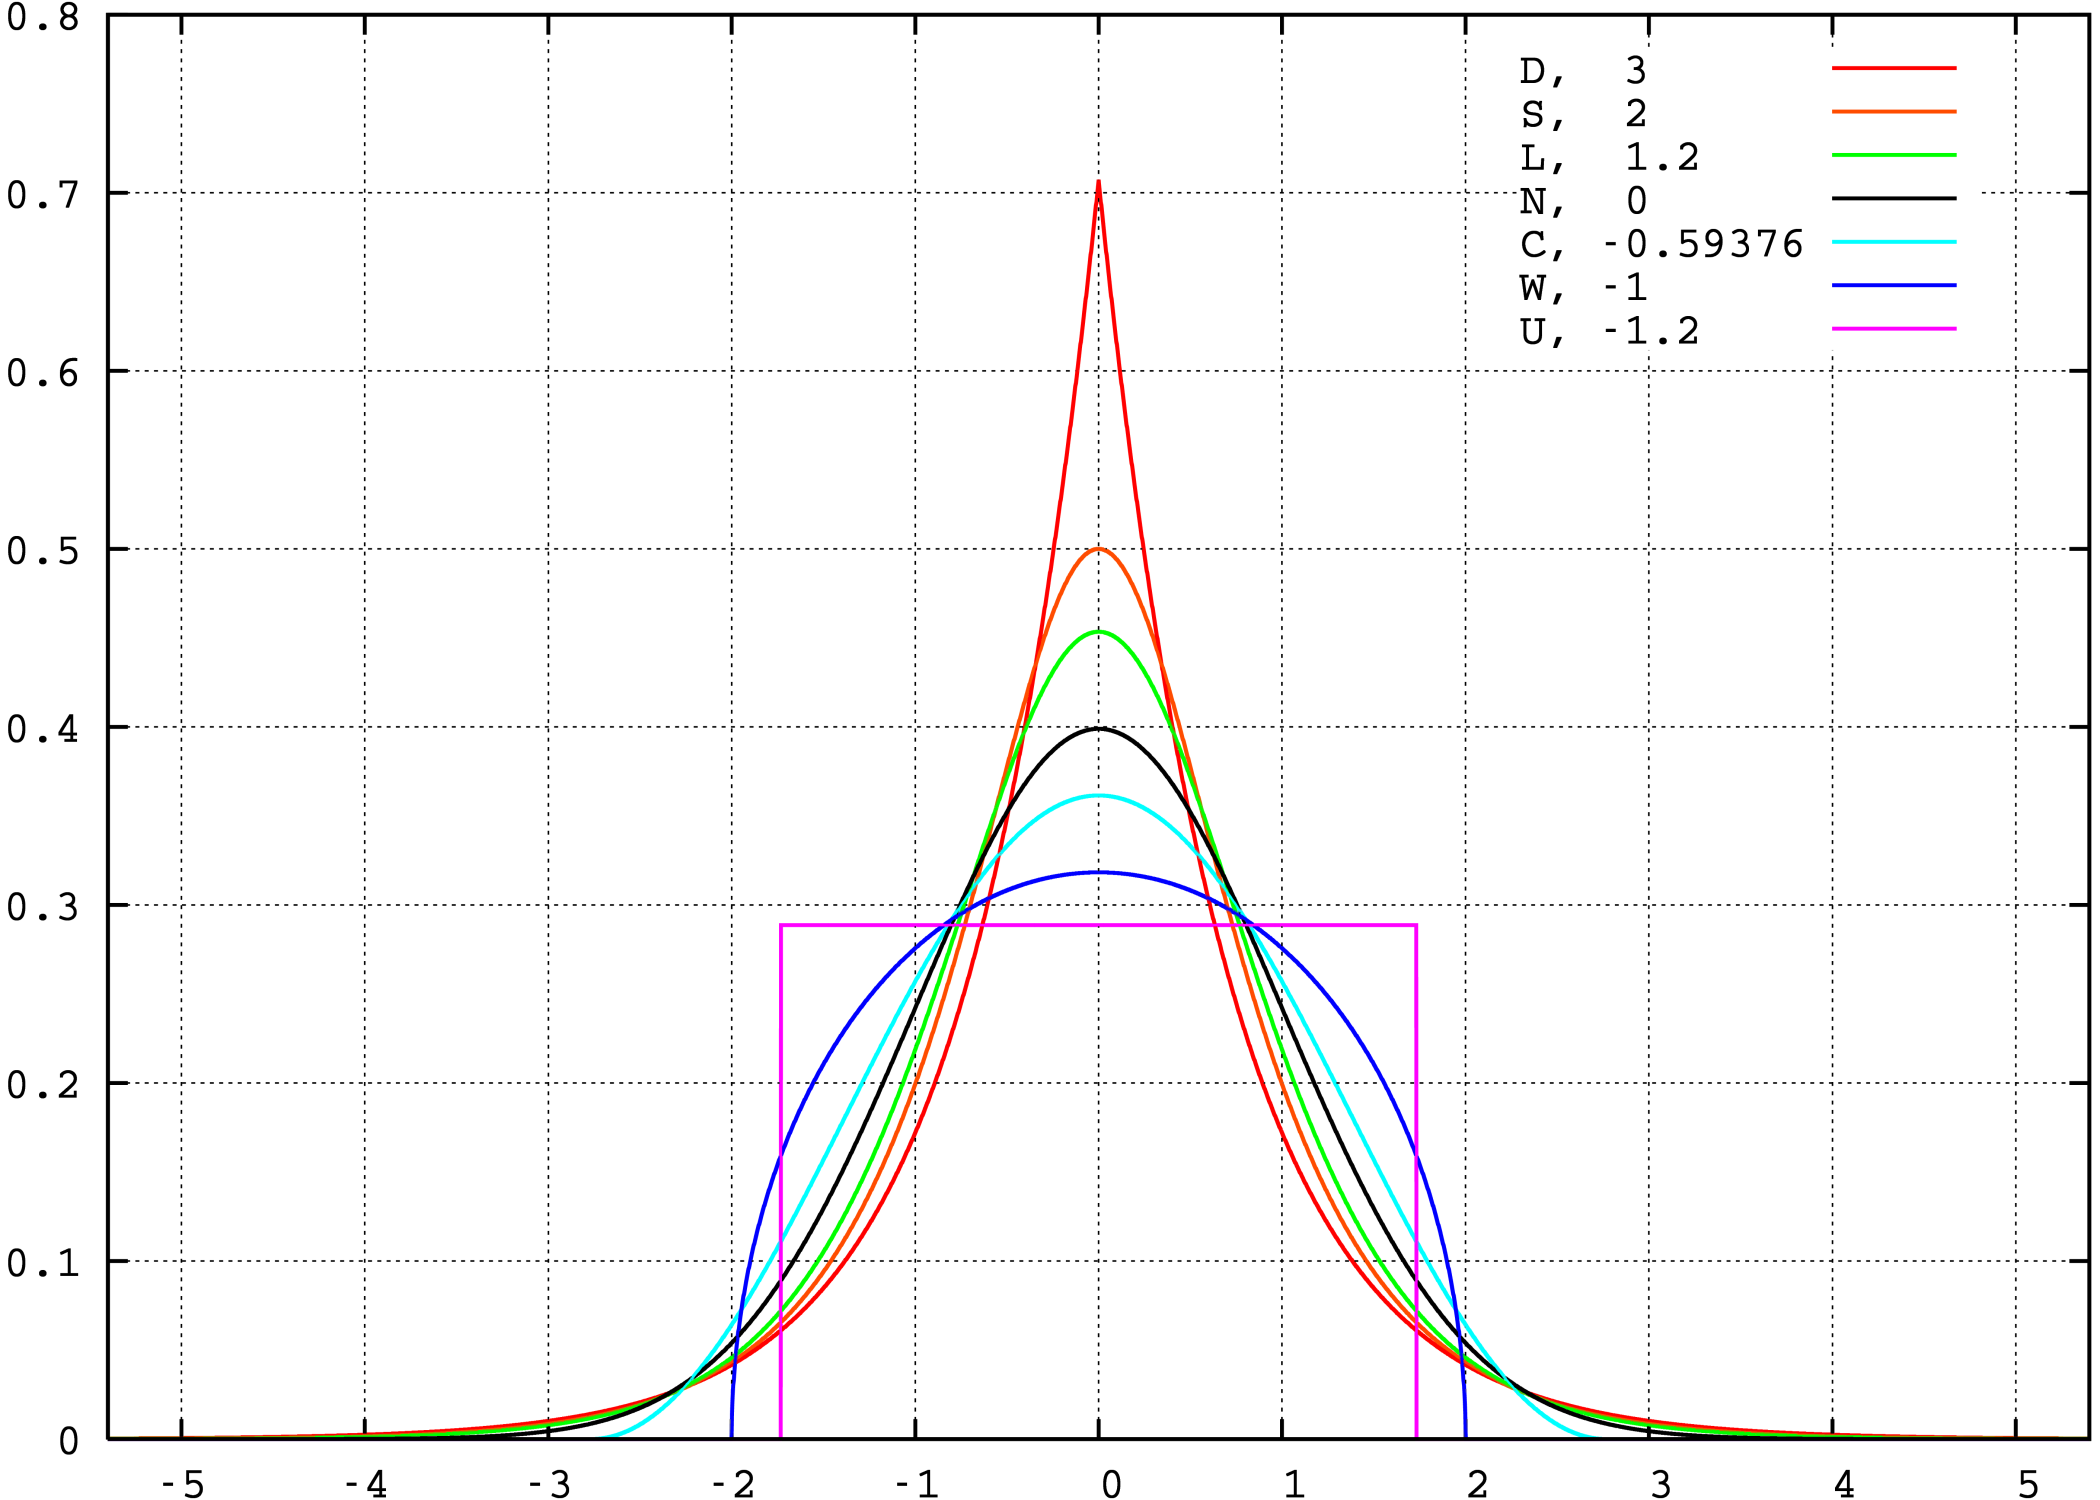
\includegraphics[width=0.8\linewidth]{kurt.png}
\end{frame}
\begin{frame}{Как выглядит распределение?}
Коэффициенты эксцесса и асимметрии сильно зависят от размера выборки и дают сбои, если выборка не унимодальна. Визуальную оценку типа распределения можно сделать по следующим графикам:\\
\begin{figure}
  \centering
  \caption{library("fitdistrplus")}
  \subfloat[descdist(x)]{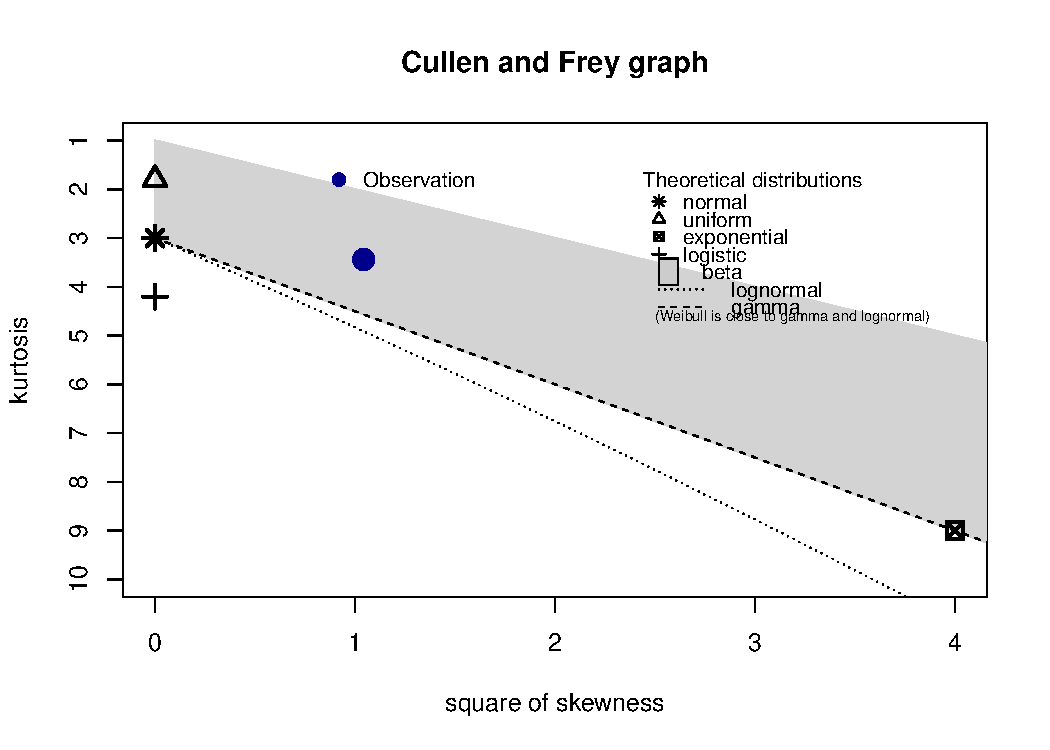
\includegraphics[width=0.48\linewidth]{descdist.pdf}}~
  \subfloat[descdist(x, discrete = T)]{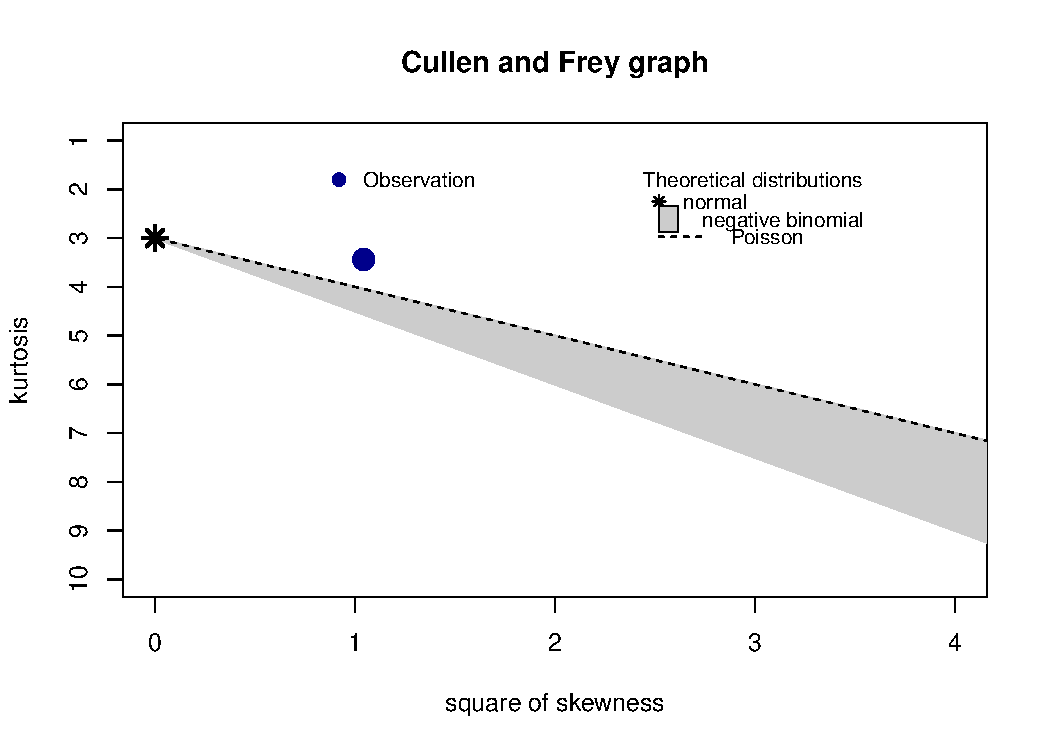
\includegraphics[width=0.48\linewidth]{descdist2.pdf}}
\end{figure}
\end{frame}
\begin{frame}{Как сравнивать два распределения?}
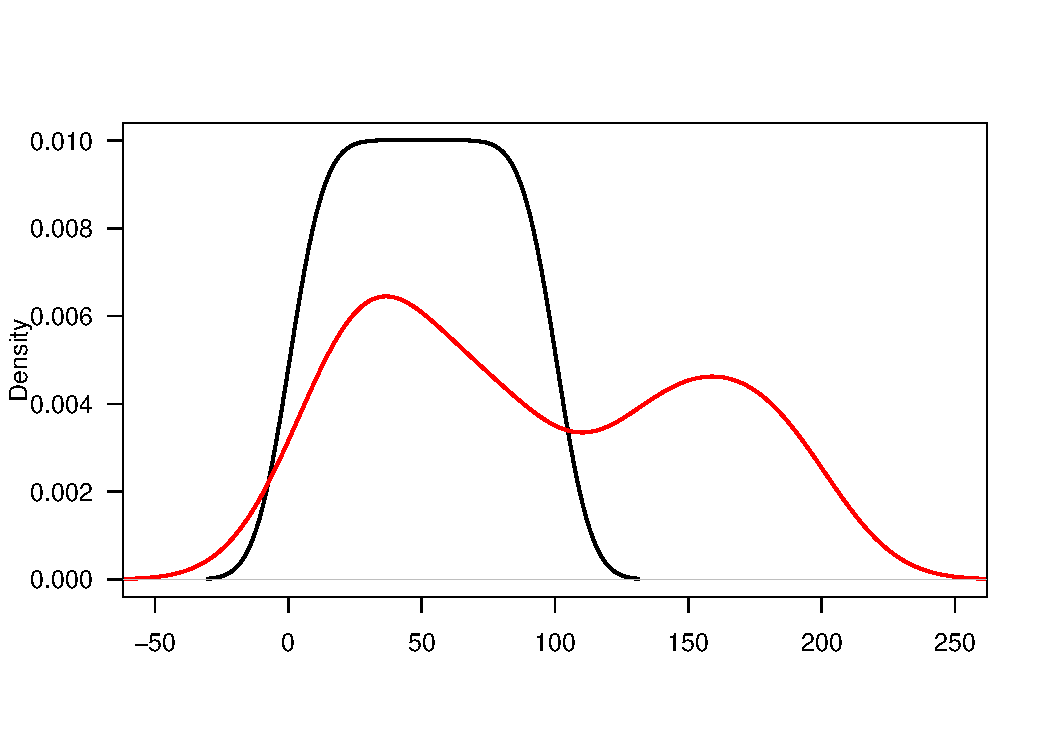
\includegraphics[width=0.62\linewidth]{1density.pdf}\pause \\
\scriptsize \verb"scale(x)" \normalsize \hfill \# z-преобразование\\
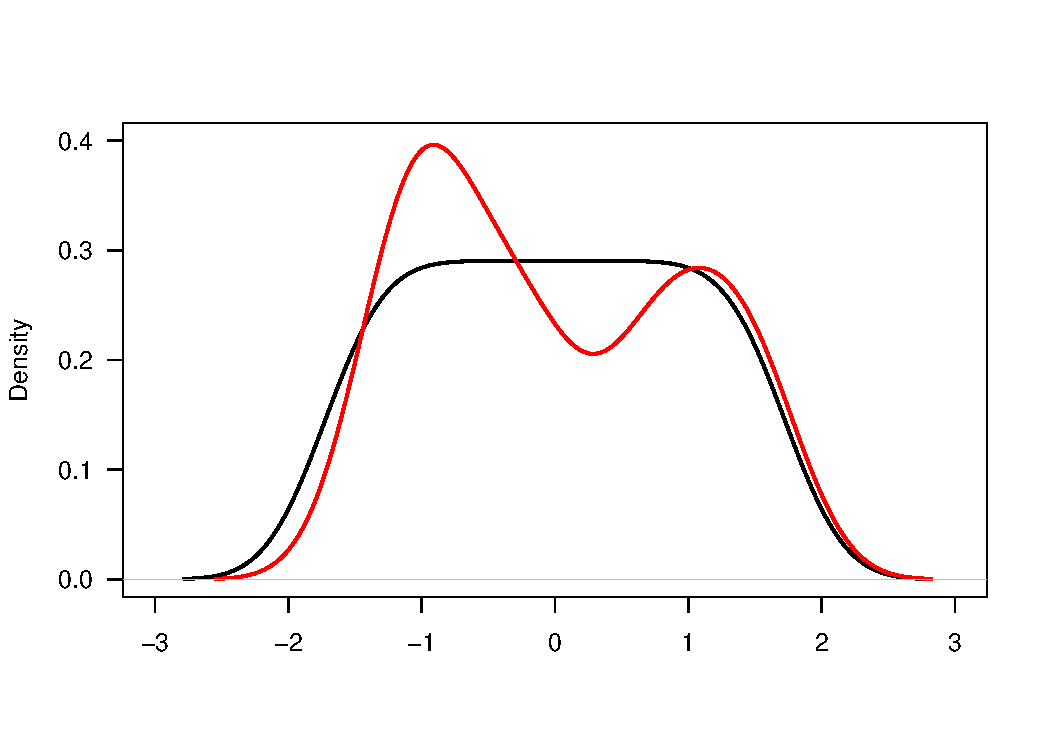
\includegraphics[width=0.62\linewidth]{2density.pdf}
\end{frame}
\section{разведочный анализ данных}
\begin{frame}{Garbage in — garbage out}
\begin{itemize}
\mytem Данные получить \textbf{\color{red!13!blue}{легко}}.
\mytem Скормить полученное компьютеру \textbf{\color{red!13!blue}{тоже легко}}. \pause
\item[\texttt{\symbol{"1F63F}}] \textbf{\color{red!13!blue}{Тяжело}} помнить, как тот или иной метод работает и какие требования предъявляет к анализируемым данным.\bigskip \pause
\item[$\Rightarrow$] Следует проводить \textbf{\color{red!13!blue}{разведочный анализ данных}}. \pause
\begin{itemize}
\item \color{red!13!blue}{визуализация}
\item {\color{red!13!blue}{формальные статистические тесты}}
\end{itemize}
В некоторых работах по статистике можно встретить предостережения относительно некоторых тестов на нормальность и аргументы в пользу графических методов. \bigskip \pause
\item[] В работе \citep{zuur10} разработан \textbf{\color{red!13!blue}{протокол разведочного анализа данных}}.
\end{itemize}
\end{frame}
\begin{frame}{Разведочный анализ данных \citep{zuur10}}
\begin{itemize}
\mytem \textbf{Outliers} \hfill \textit{boxplot and Cleveland dotplot}
\mytem \textbf{Homogeneity} \hfill \textit{conditional boxplot}
\mytem \textbf{Normality} \hfill \textit{histogram or QQ-plot}
\mytem \textbf{Zeros in data} \hfill \textit{frequency plot or corrgram}
\mytem \textbf{Collinearity} \hfill \textit{VIF and scatterplots correlation and PCA}
\mytem \textbf{Relationships between variables} \hfill \textit{multi-panel scatterplots, \\ \hfill conditional boxplots}
\mytem \textbf{Interactions} \hfill \textit{coplots}
\mytem \textbf{Independence} \hfill \textit{ACF and varlogram, plot versus time/space}
\end{itemize}
\end{frame}
\section{типология}
\begin{frame}
\vfill
Statistics are used much like a drunk uses a lamppost: for support, not illumination.\\ \hfill A.E. Housman (commonly attributed to Andrew Lang)\\
\vfill
частотная vs. байесовская статистики \\
A frequentist uses impeccable logic to answer the wrong question, while a Bayesean answers the right question by making assumptions that nobody can fully believe in.\\ \hfill P. G. Hammer\\
\hfill {\footnotesize (все так пишут, сам я первоисточника не нашел\dots)}
\vfill
параметрические vs. непараметрические
\vfill
одновыборочные vs. двухвыборочные vs. многовыборочные тесты
\vfill
парные vs. непарные тесты
\vfill
односторонние vs. двусторонние
\end{frame}
\section{одновыборочные}
\begin{frame}{Одновыборочные тесты (one-sample tests)}
\vfill
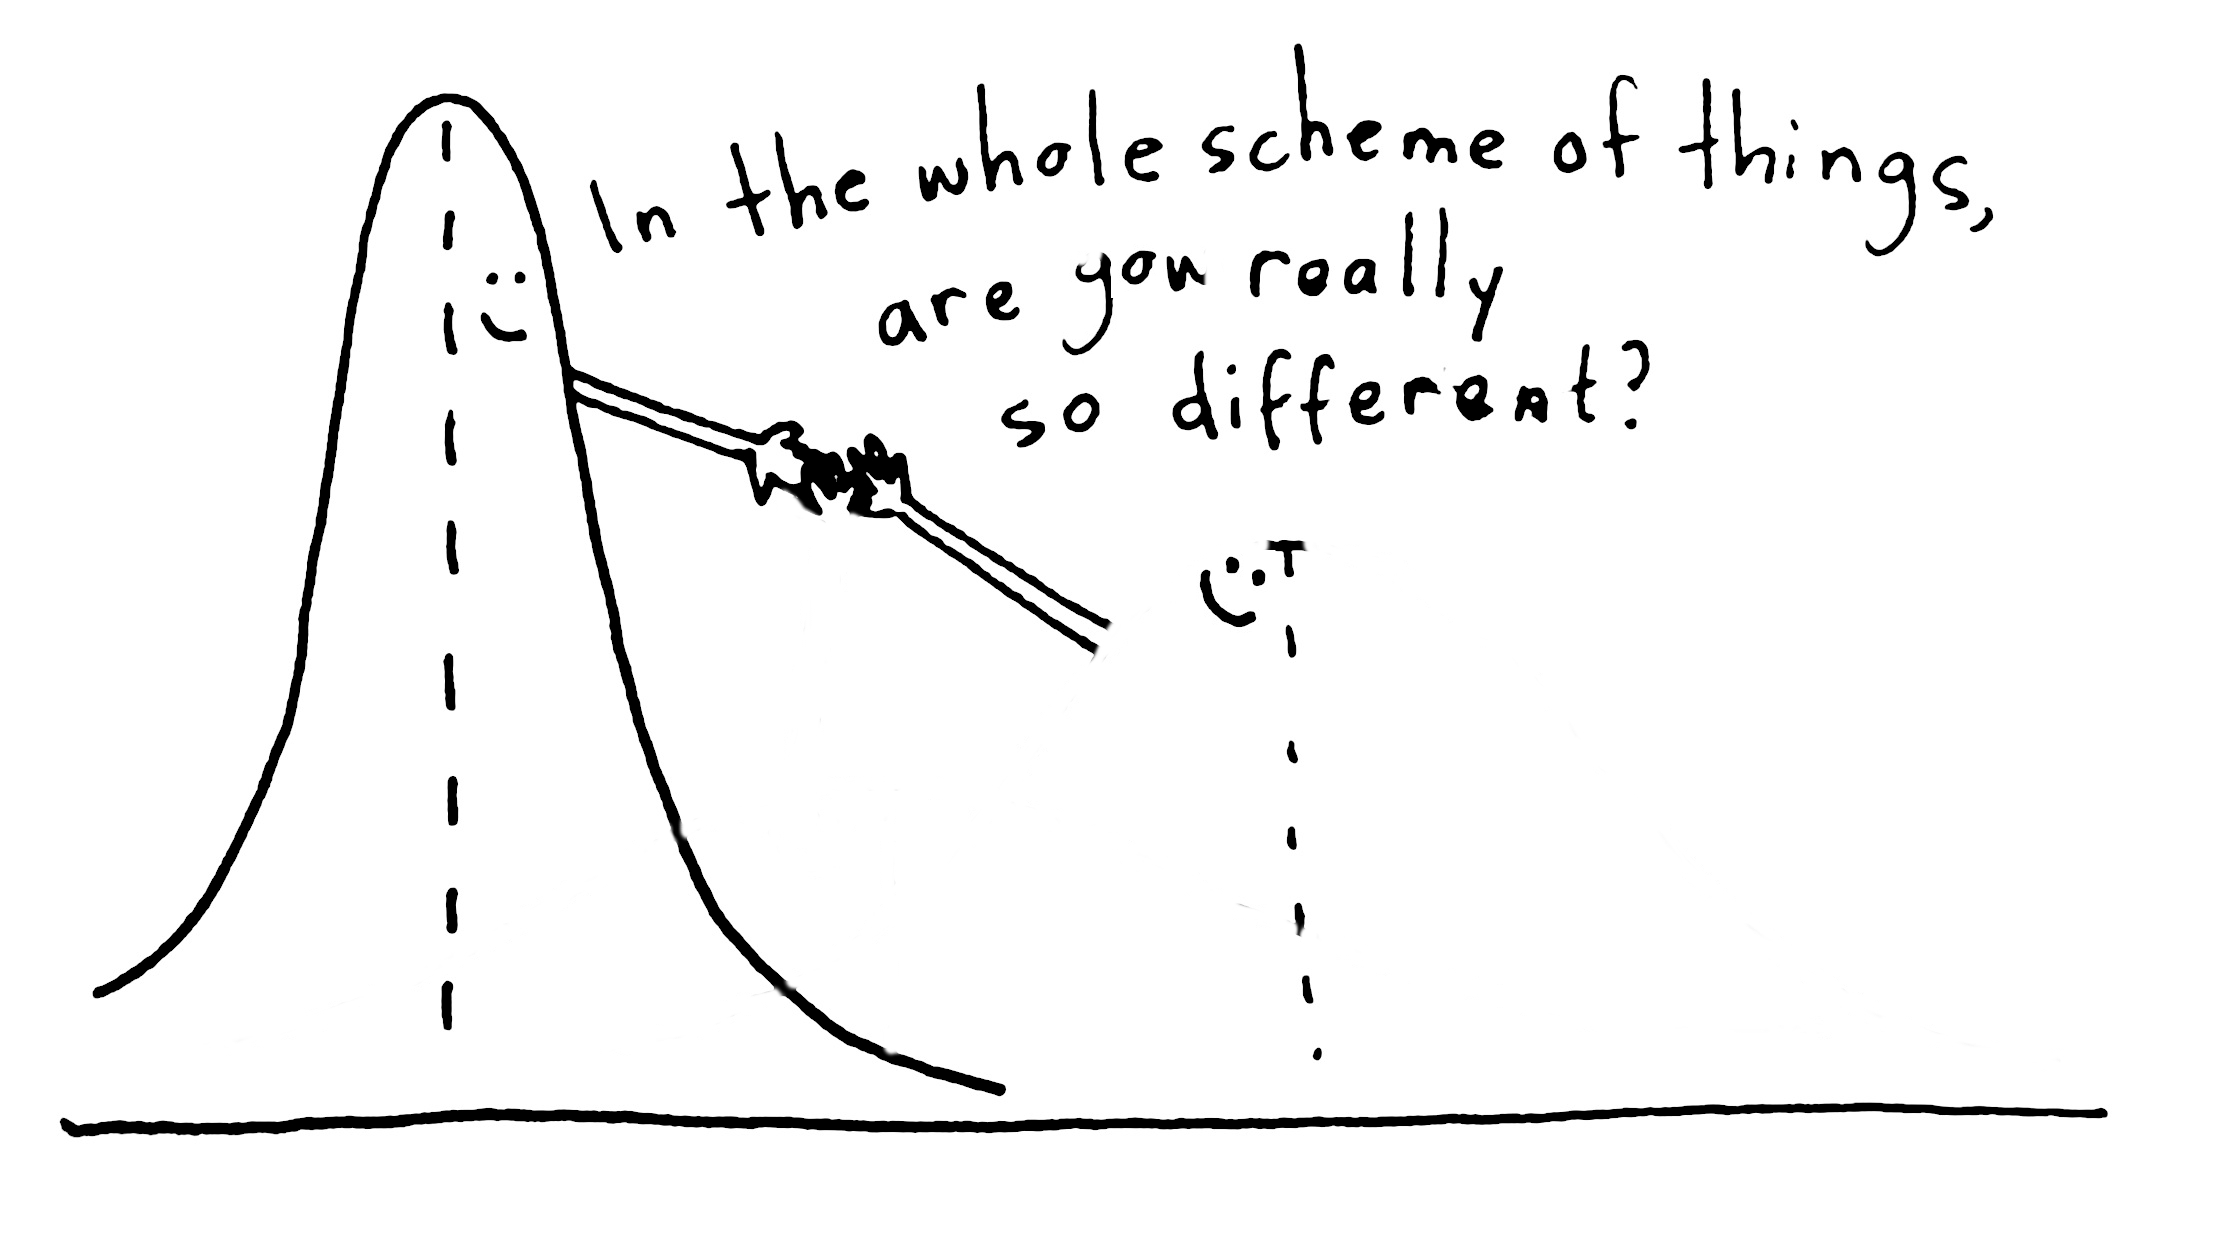
\includegraphics[width=\linewidth]{onesample.jpg}
\end{frame}
\subsection{доверительный инт.}
\begin{frame}{Задача 1: доверительный интервал}
У носителей деревни диалектные формы распределены по-разному, у некоторых — много, у некоторых —  мало или вообще отсутствуют. Из индивидуальных интервью с $n$ носителей из середины были взяты по 30 минут и измерялось количество диалектных форм. В среднем в интервью встречается $g$ диалектных черт со стандартным отклонением $s$. Что мы можем сказать о средней у всех носителей деревни? \pause 
\vfill
тип данных: количественный\\
тип теста: одновыборочный,\\
непараметрический,\\
непарный
\end{frame}
\begin{frame}{Доверительный интервал}
\begin{center}
\vspace{-4mm}
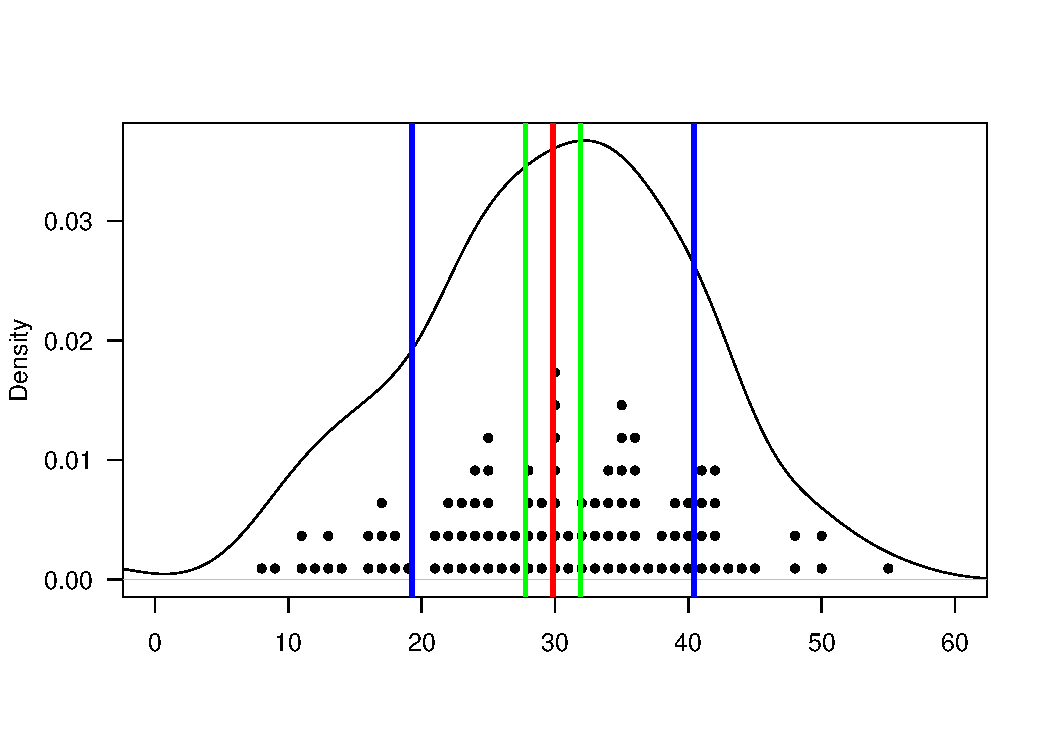
\includegraphics[width=0.71\linewidth]{confint.pdf}
{\Large \hfill \underline{для x > 30}}
\end{center}
\begin{itemize}
\mytem {\color{red}{mean(x) \hfill \# среднее}}
\mytem \alert{sd(x) \hfill \# стандартное отклонение}
\mytem sd(x)/sqrt(x)\hfill \# стандартная ошибка среднего
\mytem library("plotrix"); std.error(x) \hfill \# стандартная ошибка среднего
\mytem {\color{green}{mean(x) $\pm$ 1.96*std.error(x) \hfill \# 95\% доверительный интервал}}
\mytem mean(x) $\pm$ 2.58*std.error(x) \hfill \# 99\% доверительный интервал
\end{itemize}
K. Magnusson создал \alert{\href{http://rpsychologist.com/d3/CI/}{визуализацию доверительных интервалов}}.
\bigskip
\end{frame}
\begin{frame}{Задача 2: доверительный интервал}
Из \href{https://www.internationalphoneticassociation.org/icphs-proceedings/ICPhS2011/OnlineProceedings/RegularSession/Stepanova/Stepanova.pdf}{\alert{статьи С. Степановой}} мы знаем, что носители русского языка в среднем говорят 5.31 слога в секунду со стандартным отклонением 1,93 (мужчины 5.46 слога в секунду  со средним отклонением 2.02, женщины 5.23 слога в секунду  со средним отклонением 1.84, дети 3.86 слога в секунду со средним отклонением 1.67). Как нам определить, количество информантов $n$, которых надо опросить в данной деревне, если мы хотим, чтобы 95\% доверительный интервал был меньше 1? \pause \vfill
$$CI = \left(1.96\times \frac{sd}{\sqrt{n}}\right)\times 2$$ \vfill
$$n > \left(\left(\frac{1.96\times sd}{CI}\right)\times 2\right)^2$$ \vfill
$$n > 57.2383$$
\end{frame}
\begin{frame}{Задача 2: доверительный интервал}
Чем больше элементов в выборке, тем меньше доверительный интервал. \\
\begin{center}
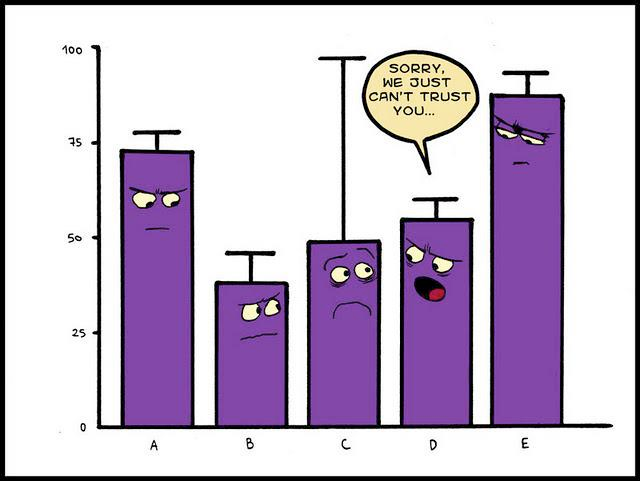
\includegraphics[width=0.8\linewidth]{conf.png}
\end{center}
\end{frame}
\begin{frame}{Как рисовать доверительные интервалы? R base}
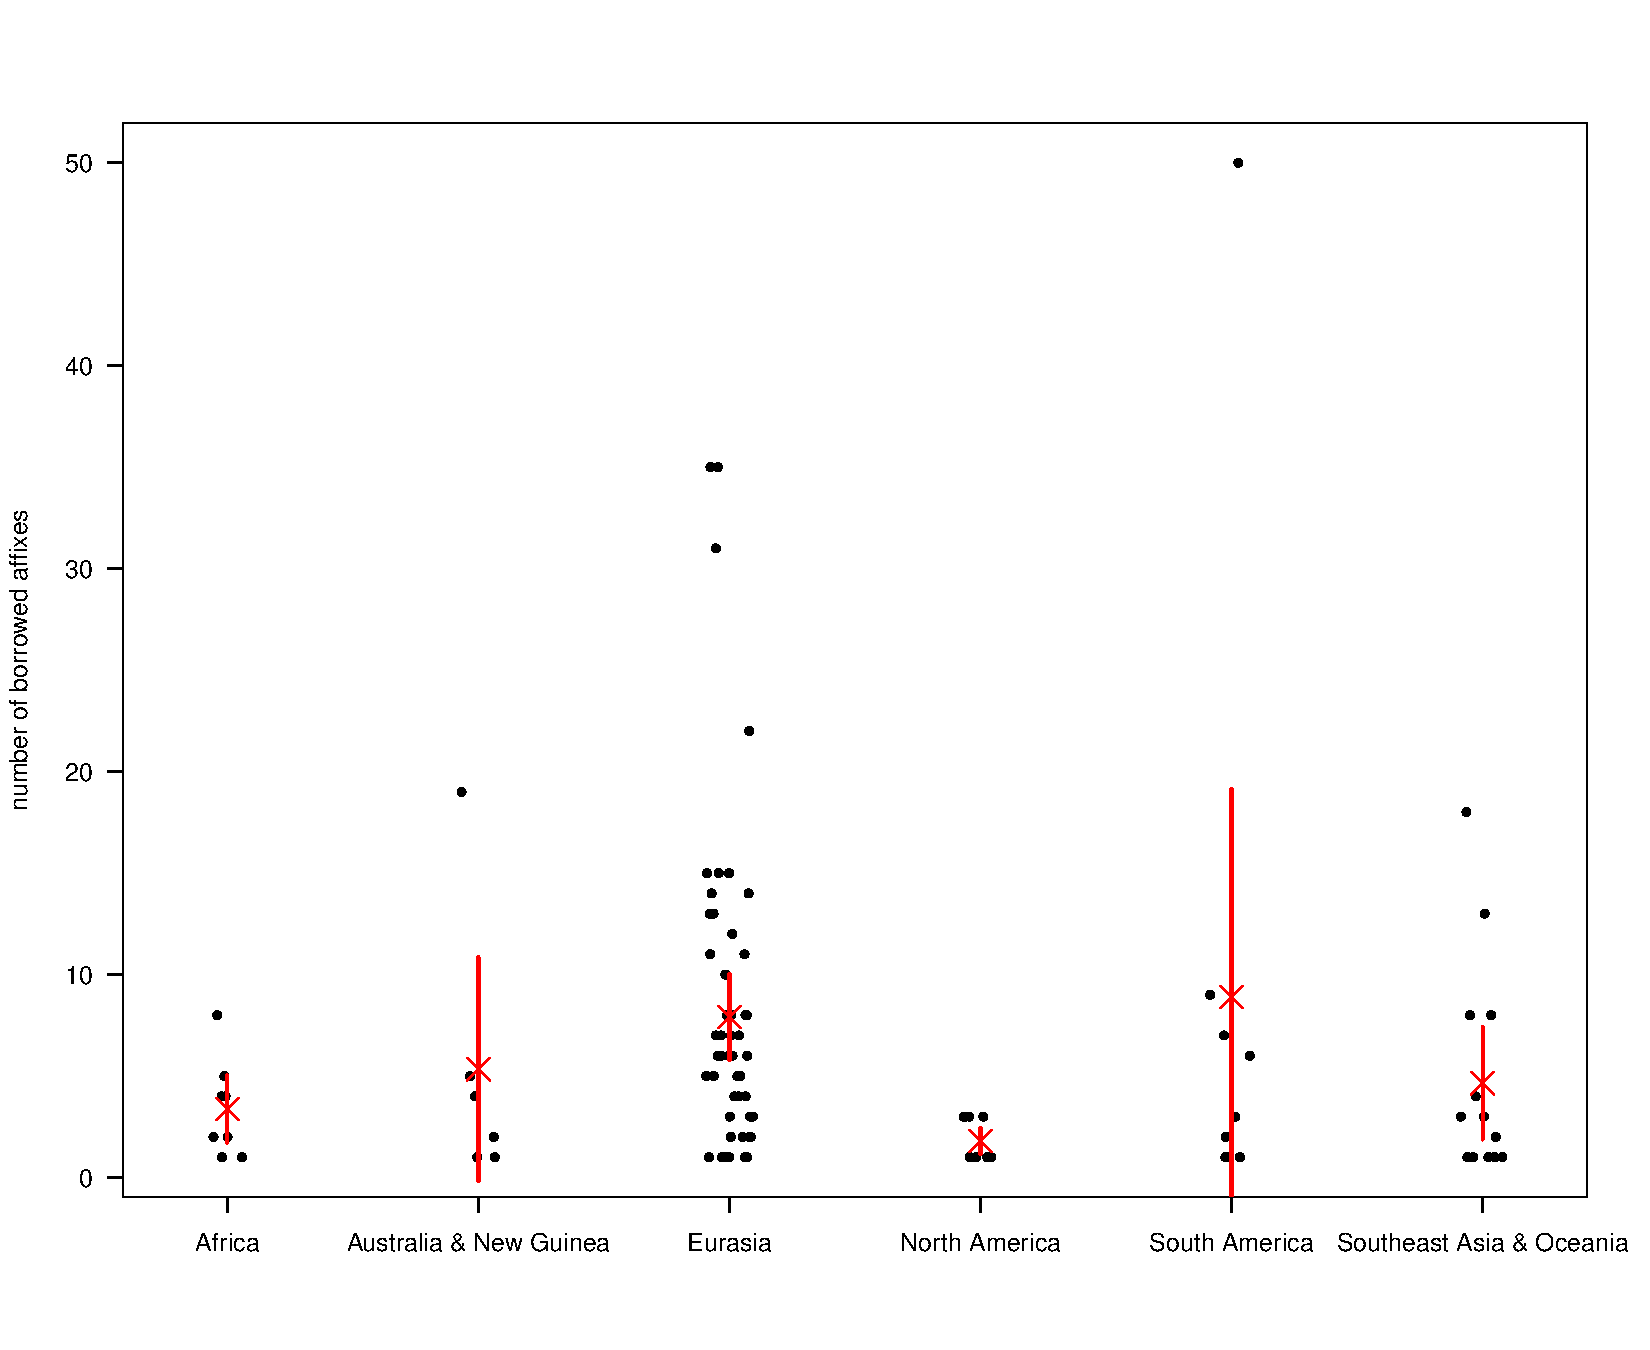
\includegraphics[width=0.92\linewidth]{rbase}
\end{frame}
\begin{frame}{Как рисовать доверительные интервалы? R base}
\scriptsize
\begin{alltt}
library("plotrix")\\
a <- read.csv("http://goo.gl/Vlvc5M") \hfill \# качаем базу данных AfBo\\
result <- cbind.data.frame(\hfill \# создадим дата фрейм\\
aggregate(number.of.borrowed.affixes \textasciitilde\ Area, a, mean), \hfill \# со средним\\
                           aggregate(number.of.borrowed.affixes \textasciitilde\ Area, a, std.error)) \hfill \# и ст. ошибк.\\
names(result)[c(2, 4)] <- c("mean"{}, "std.error")\hfill \# переименуем столбцы\medskip\\
stripchart(a\$number.of.borrowed.affixes \textasciitilde\ a\$Area, \hfill \# рисуем данные\\
           las = 1, pch = 20, method = "jitter"{}, vertical = T,\\
           ylab = "number of borrowed affixes")\hfill \# переименуем ось \medskip\\
points(result\$mean, pch = 4, cex = 2, col = "red") \hfill \# рисуем средние\\
\# нарисуем доверительный интервал\\
\alert{segments(x0 = 1:6, x1 = 1:6,\\
         y0 = result\$mean-1.96*result\$std.error,\\
         y1 = result\$mean+1.96*result\$std.error,\\
         lwd = 2, col = "red")}
\end{alltt}
\normalsize
\end{frame}
\begin{frame}{Как рисовать доверительные интервалы? ggplot2}
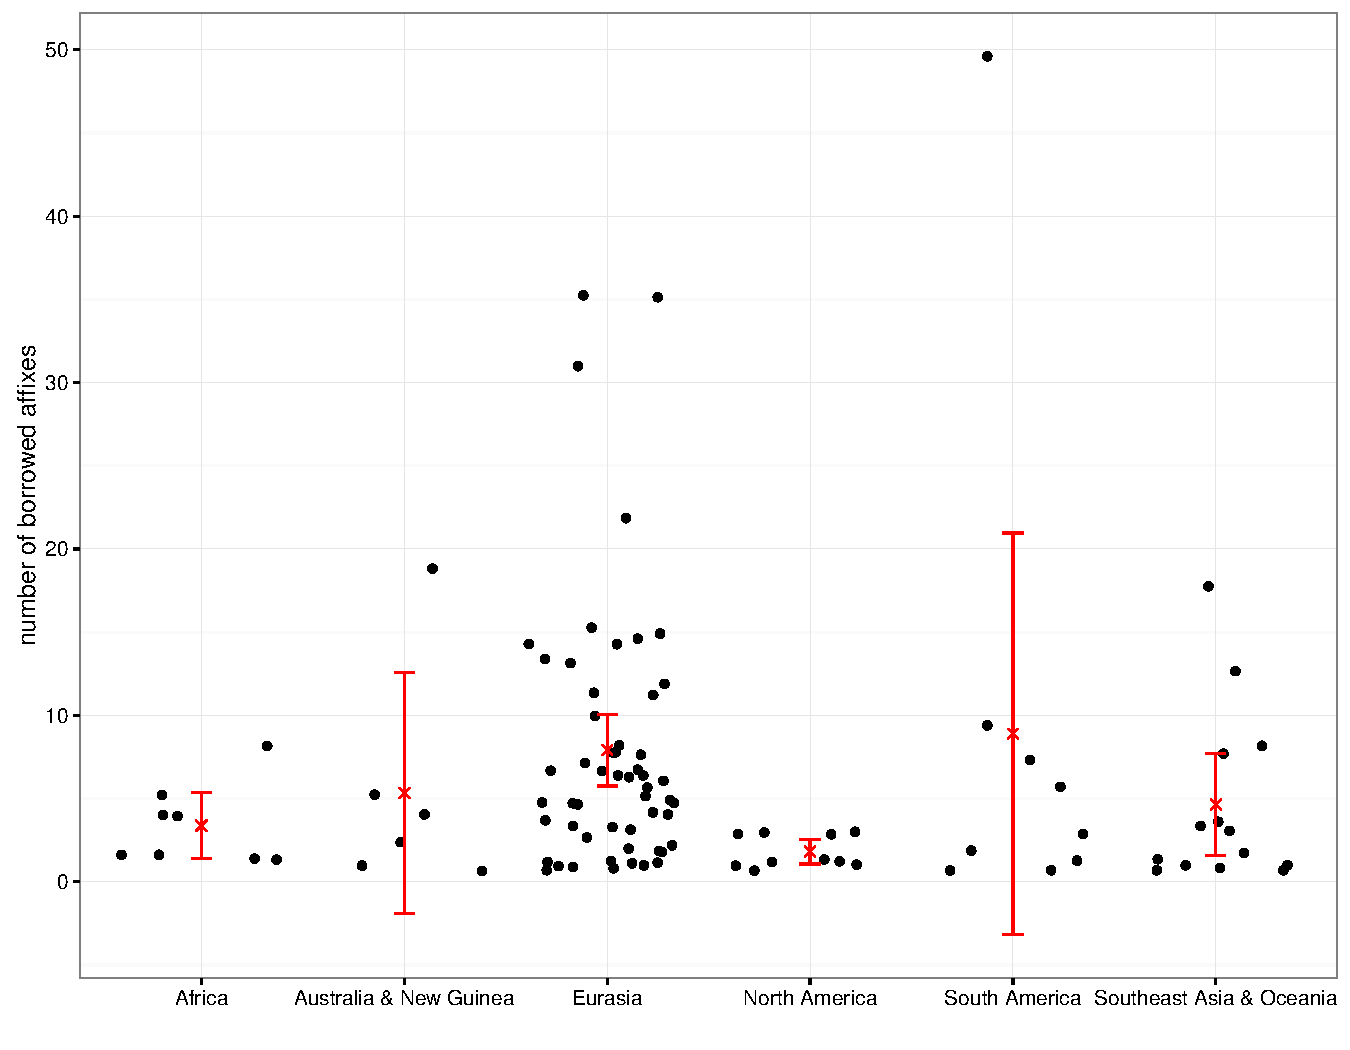
\includegraphics[width=0.97\linewidth]{ggplot}
\end{frame}
\begin{frame}{Как рисовать доверительные интервалы? ggplot2}
\scriptsize
\begin{alltt}
library("plotrix")\\
library("ggplot2")\\
a <- read.csv("http://goo.gl/Vlvc5M") \hfill \# качаем базу данных AfBo\\
result <- cbind.data.frame(\hfill \# создадим дата фрейм\\
aggregate(number.of.borrowed.affixes \textasciitilde\ Area, a, mean), \hfill \# со средним\\
                           aggregate(number.of.borrowed.affixes \textasciitilde\ Area, a, std.error)) \hfill \# и ст. ошибк.\\
names(result)[c(2, 4)] <- c("mean"{}, "std.error")\hfill \# переименуем столбцы\medskip\\
ggplot(a, aes(a\$Area, a\$number.of.borrowed.affixes))+\\
  geom\_jitter()+\hfill \# нарисуем данные\\
    xlab("")  +\\
  ylab("number of borrowed affixes")+\hfill \# переименуем ось\\
  theme\_bw()\\
stat\_summary(fun.y = mean, geom = "point"{}, \hfill \# рисуем средние\\
   size = 2, col = "red"{}, shape = 4)+\\
\alert{stat\_summary(fun.data = mean\_cl\_normal, \\
 geom = "errorbar"{}, \hfill \# рисуем доверительный интервал\\
width = 0.1, col = "red")}\\
\end{alltt}
\normalsize
\end{frame}
\subsection{t-тест}
\begin{frame}{Задача 3: одновыборочный t-тест}
Из \href{https://www.internationalphoneticassociation.org/icphs-proceedings/ICPhS2011/OnlineProceedings/RegularSession/Stepanova/Stepanova.pdf}{\alert{статьи С. Степановой}} мы знаем, что носители русского языка в среднем говорят 5.31 слога в секунду со стандартным отклонением 1,93 (мужчины 5.46 слога в секунду  со средним отклонением 2.02, женщины 5.23 слога в секунду  со средним отклонением 1.84, дети 3.86 слога в секунду со средним отклонением 1.67). Мы опросили 20 носителей деревни N и выяснили, что средняя равна 4.198775, а стандартное отклонение равно 1.976299. Является ли данная разница статистически значимой?
\vfill
тип данных: количественный\\
тип теста: одновыборочный,\\
требует нормального распределения\\
непарный
\end{frame}
\begin{frame}{Формулировка гипотезы}
Классические статистические тесты сравнивают два или более набора данных. Чаще всего:
\begin{itemize}
\mytem  строится нулевая гипотеза (H$_0$), о том, что два набора данных могли бы происходить из одной выборки
\mytem строится альтернативная гипотеза (H$_1$), о том, что два набора данных не могли бы происходить из одной выборки
\mytem устанавливается порог статистической значимости (в лингвистике принят порог 5\%)
\mytem проводится эксперимент
\mytem а дальше предъявляется p-value — вероятность случайно получить результаты эксперимента (или отличающиеся еще больше),  если мы принимаем за истину нулевую гипотезу
\end{itemize}
\end{frame}
\begin{frame}{Формулировка гипотезы}
"Whatever the approach to formal inference, formalization of the research question as being concerned with aspects of a specified kind of probability model is clearly of critical importance. It translates a subject-matter question into a formal statistical question and that translation must be reasonably faithful and, as far as is feasible, the consistency of the model with the data must be checked. {\color{red!13!blue}{\textbf{How this translation from subject-matter problem to statistical model is done is often the most critical part of an analysis}}}. Furthermore, all formal representations of the process of analysis and its justification are at best idealized models of an often complex chain of argument". \\
\hfill \cite[197]{cox06}
\end{frame}
\begin{frame}{Как интерпретировать p-value?}
\begin{center}
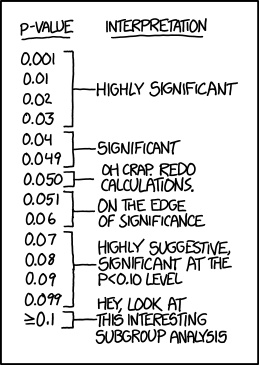
\includegraphics[width=0.45\linewidth]{ifall.png}
\end{center}
\vspace{-5mm}
If all else fails, use "significant at a p>0.05 level"\ and hope no one notices.
\\
\href{https://xkcd.com/1478/}{\alert{Комикс xkcd p-values}}. \href{http://www.explainxkcd.com/wiki/index.php/P-Values}{\alert{Объяснение}}.
\end{frame}
\begin{frame}{Задача 3: одновыборочный t-тест}
Из \href{https://www.internationalphoneticassociation.org/icphs-proceedings/ICPhS2011/OnlineProceedings/RegularSession/Stepanova/Stepanova.pdf}{\alert{статьи С. Степановой}} мы знаем, что носители русского языка в среднем говорят 5.31 слога в секунду со стандартным отклонением 1,93 (мужчины 5.46 слога в секунду  со средним отклонением 2.02, женщины 5.23 слога в секунду  со средним отклонением 1.84, дети 3.86 слога в секунду со средним отклонением 1.67). Мы опросили 20 носителей деревни N и выяснили, что средняя равна 4.198775, а стандартное отклонение равно 1.976299. Является ли данная разница статистически значимой?
\vfill
\scriptsize
\begin{alltt}
\alert{t.test(a, mu = 5.31)} \hfill \# первое — вектор значений, второе — среднее\medskip\\
One Sample t-test\\
data:  a\\
\alert{t = -2.5146, df = 19, p-value = 0.02108}\\
alternative hypothesis: true mean is not equal to 5.31\\
95 percent confidence interval:\\
 3.273838 5.123711 \hfill \# CI для среднего переменной a\\
sample estimates:\\
mean of x \\
 4.198775 
\end{alltt}
\normalsize
\end{frame}
\begin{frame}{Задача 4: нормально ли распределение?}
\begin{center}
\vspace{-4mm}
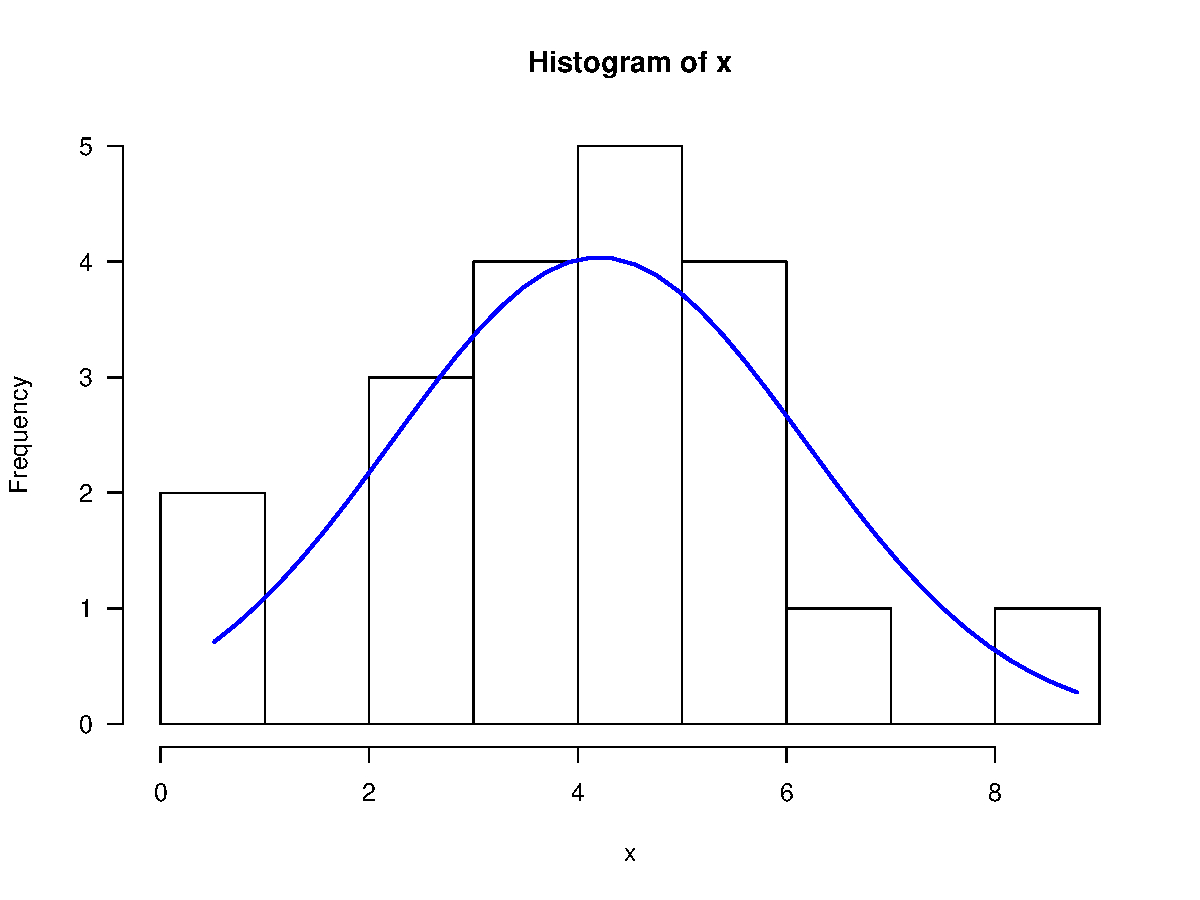
\includegraphics[width=0.74\linewidth]{normhist.pdf}
\end{center}
\scriptsize
\vfill
\begin{alltt}
h <- hist(x, las = 1) \hfill \# записывает параметры \\
xfit <- seq(min(x),max(x),length=40)  \hfill \# создает выборку \\
yfit <- dnorm(xfit,mean=mean(x),sd=sd(x))  \hfill \# получает  параметры \\
yfit <- yfit*diff(h\$mids[1:2])*length(x)  \\
lines(xfit, yfit, col="blue", lwd=2) \hfill \# рисует результат \\
\end{alltt}
\normalsize
\end{frame}
\begin{frame}{Задача 4: нормально ли распределение?}
\begin{center}
\vspace{-4mm}
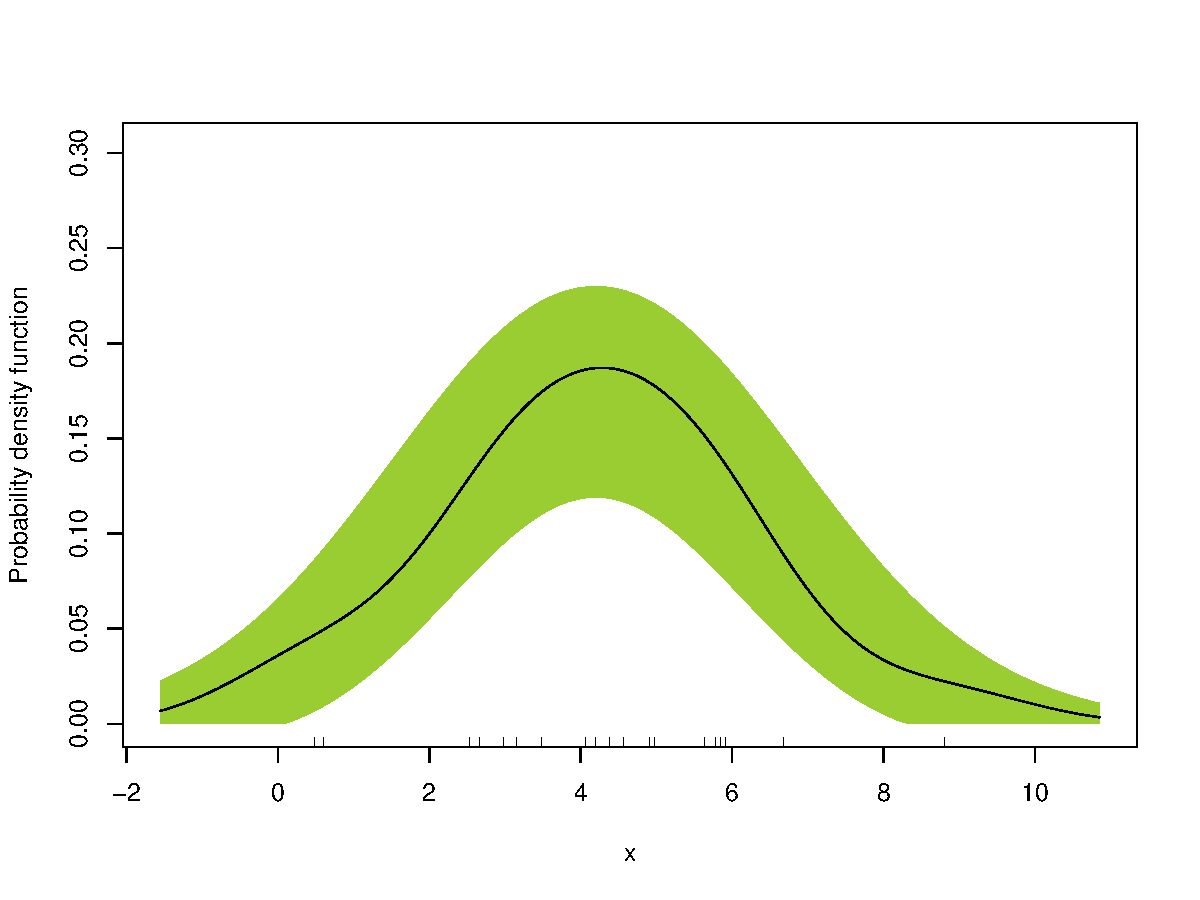
\includegraphics[width=0.85\linewidth]{normrug.pdf}
\end{center}
\scriptsize
\vfill
\begin{alltt}
library(sm)\\
sm.density(x, model = "Normal", col.band="yellowgreen")
\end{alltt}
\normalsize
\end{frame}
\begin{frame}{Задача 4: нормально ли распределение?}
\begin{center}
\vspace{-4mm}
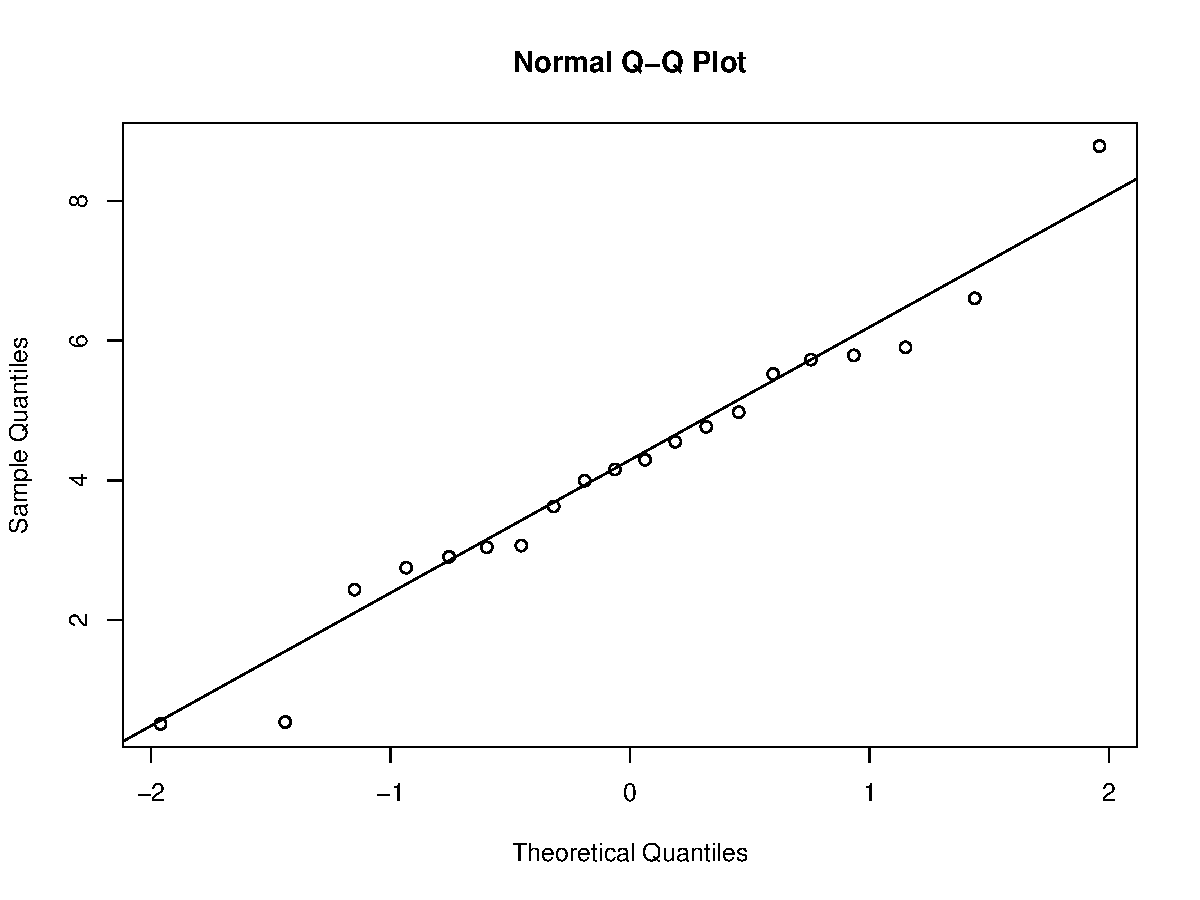
\includegraphics[width=0.85\linewidth]{qqplot.pdf}
\end{center}
\scriptsize
\vfill
\begin{alltt}
qqplot(x)\\
qqline(x)
\end{alltt}
\normalsize
\end{frame}
\begin{frame}{Задача 4: нормально ли распределение?}
Критерий Шапиро-Уилка: \hfill если наблюдений < 60\\
H$_0$: данные распределены нормально\\
H$_1$: данные не распределены нормально
\scriptsize
\begin{alltt}
\alert{shapiro.test(x)}\medskip\\
Shapiro-Wilk normality test\\
data:  x\\
\alert{W = 0.9718, p-value = 0.7923}
\end{alltt}
\normalsize
\vfill
Одновыборочный критерий Колмогорова-Смирнова: \hfill > 60\\
\scriptsize
\begin{alltt}
\alert{ks.test(x, "pnorm")}\medskip\\
One-sample Kolmogorov-Smirnov test\\
data:  x\\
\alert{D = 0.12647, p-value = 0.0816}\\
alternative hypothesis: two-sided
\end{alltt}
\normalsize
\end{frame}
\begin{frame}{Гомоскедастичность (гомогенность) дисперсии}
\begin{figure}
  \centering
  \subfloat[гомоскедастичное\label{fig:homo}]{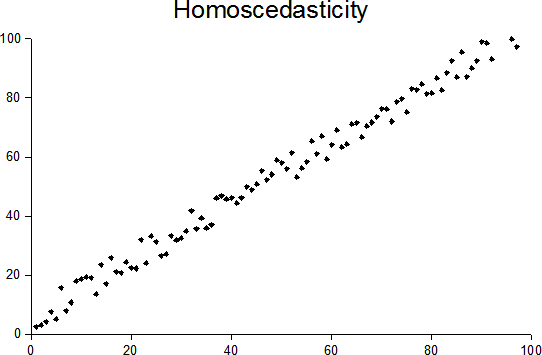
\includegraphics[width=0.45\linewidth]{Homoscedasticity.png}}\qquad
  \subfloat[гетерогедастичное\label{fig:hetero}]{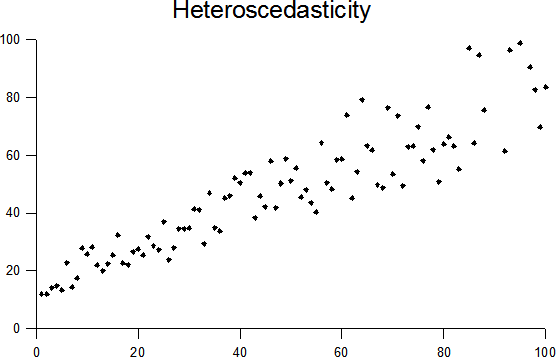
\includegraphics[width=0.45\linewidth]{Heteroscedasticity.png}}\\
распределения из Викепедии
\end{figure}
Гомоскедастичность можно проверить тестом Бартлетта:
\scriptsize
\begin{alltt}
\alert{bartlett.test(m, n)\medskip\\}
Bartlett test of homogeneity of variances\\
data:  m, n\\
\alert{Bartlett's K-squared = 2.0949, df = 1, p-value = 0.1478}
\end{alltt}
\normalsize
\end{frame}
\begin{frame}{Задача 5: сколько нужно наблюдений?}
Из \href{https://www.internationalphoneticassociation.org/icphs-proceedings/ICPhS2011/OnlineProceedings/RegularSession/Stepanova/Stepanova.pdf}{\alert{статьи С. Степановой}} мы знаем, что носители русского языка в среднем говорят 5.31 слога в секунду со стандартным отклонением 1,93 (мужчины 5.46 слога в секунду  со средним отклонением 2.02, женщины 5.23 слога в секунду  со средним отклонением 1.84, дети 3.86 слога в секунду со средним отклонением 1.67). Как нам определить, количество информантов $n$, которых надо опросить в данной деревне, если мы хотим, чтобы мы могли наблюдать разницу в 1 слог с вероятностью совершить ошибку первого рода α~0.05 и мощностью теста~0.8? \pause
\vfill
\scriptsize
\begin{alltt}
\alert{power.t.test(sig.level = 0.05, \hfill \# α\\
			power = 0.8, \hfill \# мощность теста\\
             delta = 1, \hfill \# наблюдаемая разница\\
             sd = 1.93, \hfill \# стандартное отклонение\\
              type = "one.sample"{},\\
             alternative = "one.sided")}
\medskip\\
One-sample t test power calculation \\
\alert{n = 24.44055} \\
\dots
\end{alltt}
\normalsize
\end{frame}
\subsection{критерий Уилкоксона}
\begin{frame}{Задача 6: выборка не распределена нормально?}
\scriptsize
\begin{alltt}
\alert{wilcox.test(x, mu = 5,31)}\medskip\\
Wilcoxon rank sum test\\
data:  x and 31\\
\alert{W = 0, p-value = 0.04878}\\
alternative hypothesis: true location shift is not equal to 5
\end{alltt}
\normalsize
\vfill
тип данных: количественный\\
тип теста: одновыборочный,\\
непараметрический,\\
непарный
\end{frame}
\subsection{биномиальный тест}
\begin{frame}{Задача 7: биномиальный тест}
\href{http://dict.ruslang.ru/freq.php}{В \alert{частотном словаре \citep{lyashevskaya09}}}, созданном на корпусе объемом 92 млн. словоупотреблений, существительное \textit{кенгуру} имеет абсолютную частотность 0.0000021, а предлог \textit{к} — 0.005389 (его алломорф \textit{ко} в расчет не берется). В некотором тексте, имеющем 61981 слов существительное \textit{кенгуру} встречается 58 раз, а предлог \textit{к} — 254. Каковы вероятности получить такие результаты?\\ \pause
\vfill
\footnotesize
\begin{alltt}
binom.test(x = 58, n = 61981, p = 0.0000021) \hfill \# про \textit{кенгуру} \\
binom.test(58, 61981, 0.0000021) \hfill \# про \textit{кенгуру}\\ 
binom.test(254, 61981, 0.005389) \hfill \# про \textit{к}
\end{alltt}
\normalsize
\vfill
тип данных: категориальный\\
тип теста: одновыборочный,\\
непараметрический,\\
непарный
\end{frame}
\section{двухвыборочные}
\begin{frame}{Двухвыборочные тесты (two-sample tests)}
\vfill
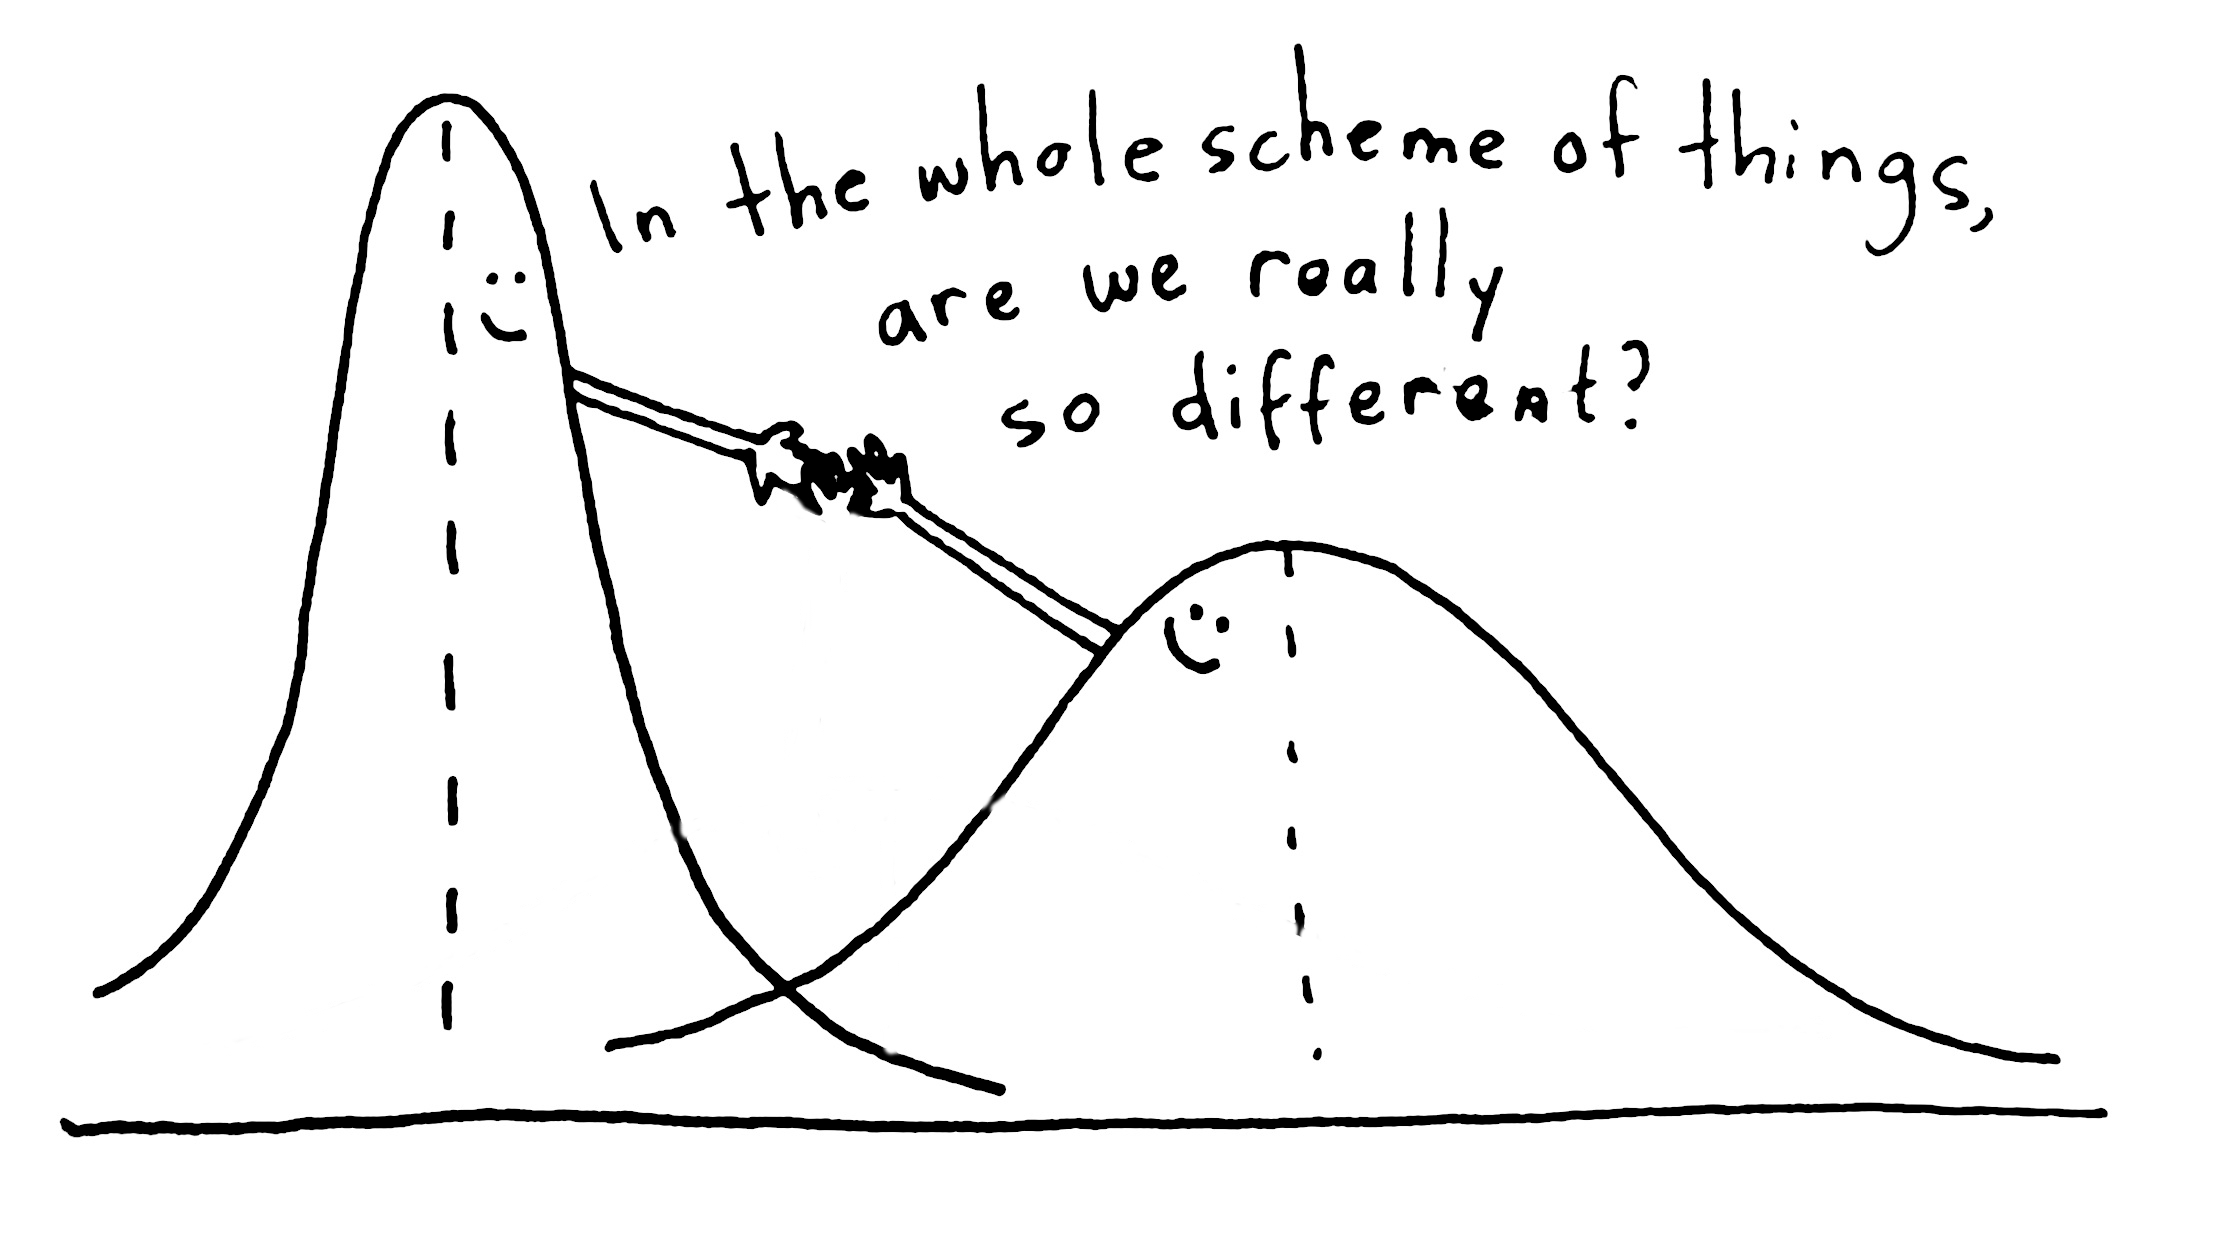
\includegraphics[width=\linewidth]{twosample.jpg}
\end{frame}
\subsection{t-тест}
\begin{frame}{Задача 8: двухвыборочный t-тест}
Из \href{https://www.internationalphoneticassociation.org/icphs-proceedings/ICPhS2011/OnlineProceedings/RegularSession/Stepanova/Stepanova.pdf}{\alert{статьи С. Степановой}} мы знаем, что носители русского языка в среднем говорят 5.31 слога в секунду со стандартным отклонением 1,93 (мужчины 5.46 слога в секунду  со средним отклонением 2.02, женщины 5.23 слога в секунду  со средним отклонением 1.84, дети 3.86 слога в секунду со средним отклонением 1.67). Является ли данная разница между мужчинами и женщинами статиститчески значимой?
\vfill
тип данных: количественный\\
тип теста: двухвыборочный,\\
требует нормального распределения и гомоскедастичности\\
непарный
\end{frame}
\begin{frame}{Задача 8: двухвыборочный t-тест}
Из \href{https://www.internationalphoneticassociation.org/icphs-proceedings/ICPhS2011/OnlineProceedings/RegularSession/Stepanova/Stepanova.pdf}{\alert{статьи С. Степановой}} мы знаем, что носители русского языка в среднем говорят 5.31 слога в секунду со стандартным отклонением 1,93 (мужчины 5.46 слога в секунду  со средним отклонением 2.02, женщины 5.23 слога в секунду  со средним отклонением 1.84, дети 3.86 слога в секунду со средним отклонением 1.67). Является ли данная разница между мужчинами и женщинами статиститчески значимой?
\vfill
\scriptsize
\begin{alltt}
\alert{t.test(a, b)} \hfill \# первое и второе — векторы значений\medskip\\
Welch Two Sample t-test\\
data:  a and b\\
\alert{t = 0.38408, df = 37.919, p-value = 0.7031}\\
alternative hypothesis: true difference in means is not equal to 0\\
95 percent confidence interval: \\
 -0.9984148  1.4659358 \hfill \# CI для величины эффекта\\
sample estimates:\\
mean of x mean of y \\
 5.465256  5.231496
\end{alltt}
\normalsize
\end{frame}
\begin{frame}{Задача 9: парный t-тест}
Влияет ли ударение на длительность гласных? В группе слов [a] и [i] встречается как под ударением, так и без (10 слов с ударным [a], 10 слов с ударным [i], 10 слов с безударным [a], 10 слов с безударным [i]). 20 носителей читают все слова, а исследовали для каждого носителя посчитали среднюю длинну ударных и безударных [a] и [i]. Есть ли статистически значимая разница между ударными и безударными гласными?
\vfill
тип данных: количественный\\
тип теста: двухвыборочный,\\
требует нормального распределения и гомоскедастичности\\
парный
\end{frame}
\begin{frame}{Задача 9: парный t-тест}
Влияет ли ударение на длительность гласных? В группе слов [a] и [i] встречается как под ударением, так и без (10 слов с ударным [a], 10 слов с ударным [i], 10 слов с безударным [a], 10 слов с безударным [i]). 20 носителей читают все слова, а исследовали для каждого носителя посчитали среднюю длинну ударных и безударных [a] и [i]. Есть ли статистически значимая разница между ударными и безударными гласными?\vfill
\scriptsize
\begin{alltt}
\alert{t.test(m, f, paired = T)}\medskip\\
Paired t-test\\
data: str and unstr\\
\alert{t = 5.9903, df = 19, p-value = 9.165e-06}\\
alternative hypothesis: true difference in means is not equal to 0\\
95 percent confidence interval:\\
18.03107 37.39799 \hfill \# CI для величины эффекта\\
sample estimates:\\
mean of the differences\\
27.71453
\end{alltt}
\normalsize
\end{frame}
\begin{frame}{Парные тесты}
Парные тесты применяют, если исследуют:
\begin{itemize}
\mytem наблюдения до/после (измерения скорости речи при первом рассказе и при пересказе)
\mytem наблюдения одного и того же объекта, полученные разными методами (например, кроссвалидация разметки)
\end{itemize}
\end{frame}
\subsection{Манн—Уитни, Уилкоксон}
\begin{frame}{Задача 9: выборки не распределена нормально?}
\scriptsize
\begin{alltt}
\alert{wilcox.test(a, b)} \hfill \# критерий Манна—Уитни\medskip\\
Wilcoxon rank sum test\\
data:  a and b\\
W = 243, p-value = 0.2534
alternative hypothesis: true location shift is not equal to 0
\end{alltt}
\normalsize
\vfill
\scriptsize
\begin{alltt}
\alert{wilcox.test(c,d, paired = T)}\hfill \# критерий Уилкоксона\medskip\\
Wilcoxon signed rank test\\
data:  c and d\\
\alert{V = 80, p-value = 0.3683}\\
alternative hypothesis: true location shift is not equal to 0
\end{alltt}
\normalsize
\vfill
Если добавить аргумент \scriptsize\verb"conf.int = T"\normalsize, то отобразится еще и  95\% доверительный интервал, в котором находится величина эффекта.
\vfill
тип данных: количественный\\
тип теста: двухвыборочный,\\
непараметрический,\\
непарный, парный\\
\end{frame}
\subsection{критерий χ²}
\begin{frame}{Задача 10: χ² (с поправкой Йейтса)}
Из интервью с носителями одной деревни произвольным образом выбрали по пол часа и посчитали кол-во реализаций диалектных форм vs. недиалектных. В результате получилось что у женщин было 107 диалектных форм vs. 93 недиалектные, а у мужчин  — 74 vs. 45.
\vfill
тип данных: категориальный\\
тип теста: двухвыборочный,\\
непараметрический,\\
непарный
\end{frame}
\begin{frame}{Задача 10: χ² (с поправкой Йейтса)}
Из интервью с носителями одной деревни произвольным образом выбрали по пол часа и посчитали кол-во реализаций диалектных форм vs. недиалектных. В результате получилось что у женщин было 107 диалектных форм vs. 93 недиалектные, а у мужчин  — 74 vs. 45. Значима ли зафиксированная разница?
\vfill
Сначала следует составить таблицу сопряженности:
\scriptsize
\begin{alltt}
\alert{table(dialect)}\hfill \# таблица сопряженности\medskip\\
\begin{tabular}{rcc}
 & \multicolumn{ 2}{c}{feature} \\ 
sex & -d & +d \\ 
f & 107 & 93 \\ 
m & 74 & 45 \\ 
\end{tabular}
\end{alltt}
\normalsize
А дальше используем тест:
\scriptsize
\begin{alltt}
\alert{chisq.test(table(dialect))}\medskip\\
Pearson's Chi-squared test with Yates' continuity correction\\
data:  table(dialect)\\
\alert{X-squared = 1.9525, df = 1, p-value = 0.1623}
\end{alltt}
\normalsize
\end{frame}
\begin{frame}{Критерий Фишера, критерий Крамера}
Иногда R может сказать:\\
\scriptsize\verb"Chi-squared approximation may be incorrect"\\ \normalsize
\vfill
Критерий χ² плохо использовать:
\begin{itemize}
\mytem если хотя бы в одной из клеток \textbf{\underline{ожидаемое значение}} меньше 5
\scriptsize\verb"chi.t <- chisq.test(a)"\normalsize\\
\scriptsize\verb"chi.t\alert{\$expected}"\normalsize
\begin{itemize}
\item[→] точный тест Фишера (\scriptsize\verb"fisher.test()"\normalsize)
\end{itemize}
\mytem если между числами есть большой разрыв\footnote[frame]{\href{http://stats.stackexchange.com/a/108914}{\alert{ "All differences are significant with a large enough sample size"}\\}}
\begin{itemize}
\item[→] проверяем величину эффекта критерием Крамера (\scriptsize\verb"cramersV()"\normalsize\ в пакете \scriptsize\verb"lsr"\normalsize)
\end{itemize}
\mytem \dots вообще таблицы сопряженности бывают разные, да и тестов куда больше см.~\citep{lydersen09}
\end{itemize}
\end{frame}
\subsection{критерий Мак Немара}
\begin{frame}{Задача 11: критерий Мак Немара}
Во время диалектологической экспедиции от 20 информантов (10 мужчин, 10 женщин) были записаны списки слов. Получилось, что мужчины произносят велярный фрикативный ɣ в 13 случаях, а велярный стоп ɡ в 43. У женщин получилось другое распределение: 19 ɣ против 37 ɡ. Является ли данная разница между мужчинами и женщинами статистически значимой?
\vfill
тип данных: категориальный\\
тип теста: двухвыборочный,\\
непараметрический,\\
парный
\end{frame}
\begin{frame}{Задача 11: критерий Мак Немара}
Во время диалектологической экспедиции от 20 информантов (10 мужчин, 10 женщин) были записаны списки слов. Получилось, что 13 информантов использовали в речи велярный фрикативный ɣ, а 22 — велярный стоп ɡ. Через 5 лет работали с теми же информантами и соотношение немного поменялось: 7 ɣ против 28 ɡ. Является ли получившаяся разница статистически значимой?
\vfill
Сначала следует составить таблицу сопряженности:
\scriptsize
\begin{alltt}
\alert{table(stopfricg)}\hfill \# таблица сопряженности\medskip\\
\begin{tabular}{rcc}
 & \multicolumn{ 2}{c}{feature} \\ 
time & fric & stop \\ 
before & 13 & 22 \\ 
after & 7 & 28 \\ 
\end{tabular}
\end{alltt}
\normalsize
А дальше используем тест:
\scriptsize
\begin{alltt}
\alert{mcnemar.test(table(stopfricg))}\medskip\\
McNemar's Chi-squared test with continuity correction\\
data:  table(stopfricg)\\
McNemar's chi-squared = 6.7586, df = 1, p-value = 0.00933\\
\end{alltt}
\normalsize
\end{frame}
\subsection{multiple testing effect}
\begin{frame}{Об эффекте множественных сравнений}
\vfill
\begin{center}
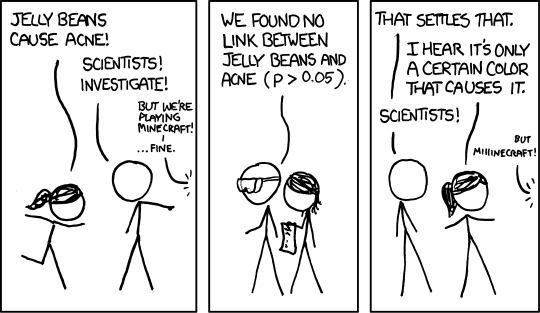
\includegraphics[width=0.8\linewidth]{jellybeanexample1.png}
\end{center}
\end{frame}
\begin{frame}{Об эффекте множественных сравнений}
\vfill
\begin{center}
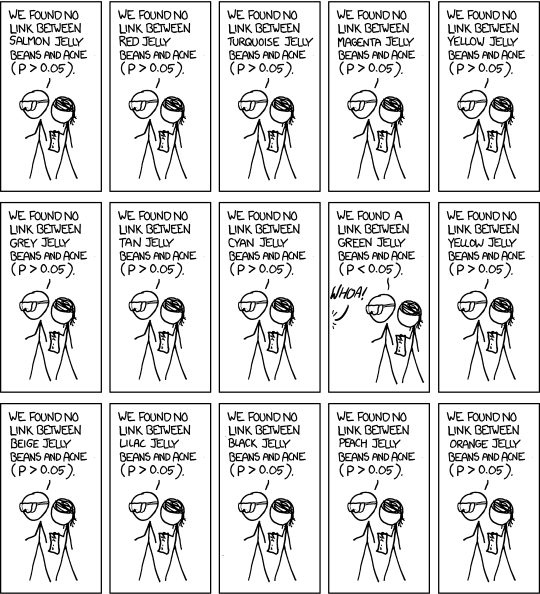
\includegraphics[width=0.65\linewidth]{jellybeanexample2.png}
\end{center}
\end{frame}
\begin{frame}{Об эффекте множественных сравнений}
\vfill

\includegraphics[width=0.8\linewidth]{jellybeanexample3.png}\\
\href{https://xkcd.com/882/}{\alert{Комикс xkcd Significant}}. \href{http://www.explainxkcd.com/wiki/index.php/882}{\alert{Объяснение}}.\\
Это называют: data dredging, data fishing, data snooping, equation fitting, p-hacking\dots
\end{frame}
\begin{frame}{Об эффекте множественных сравнений}
При проверке каждой статистической гипотезы закладывается возможность ошибки первого рода (т. е. отклонение верной нулевой гипотезы). Чем больше гипотез мы проверяем на одних и тех же данных, тем больше будет вероятность допустить как минимум одну такую ошибку.  Вероятность того, что из 21 теста (включая первый тест, без исключения цвета) не будет допущена ошибка первого рода равна 
$$P = (1-\alpha)^m = (1 - 0.05)^{21} = 0.34$$
\end{frame}
\begin{frame}{Многовыборочные тесты (multiple-sample tests)}
\vfill
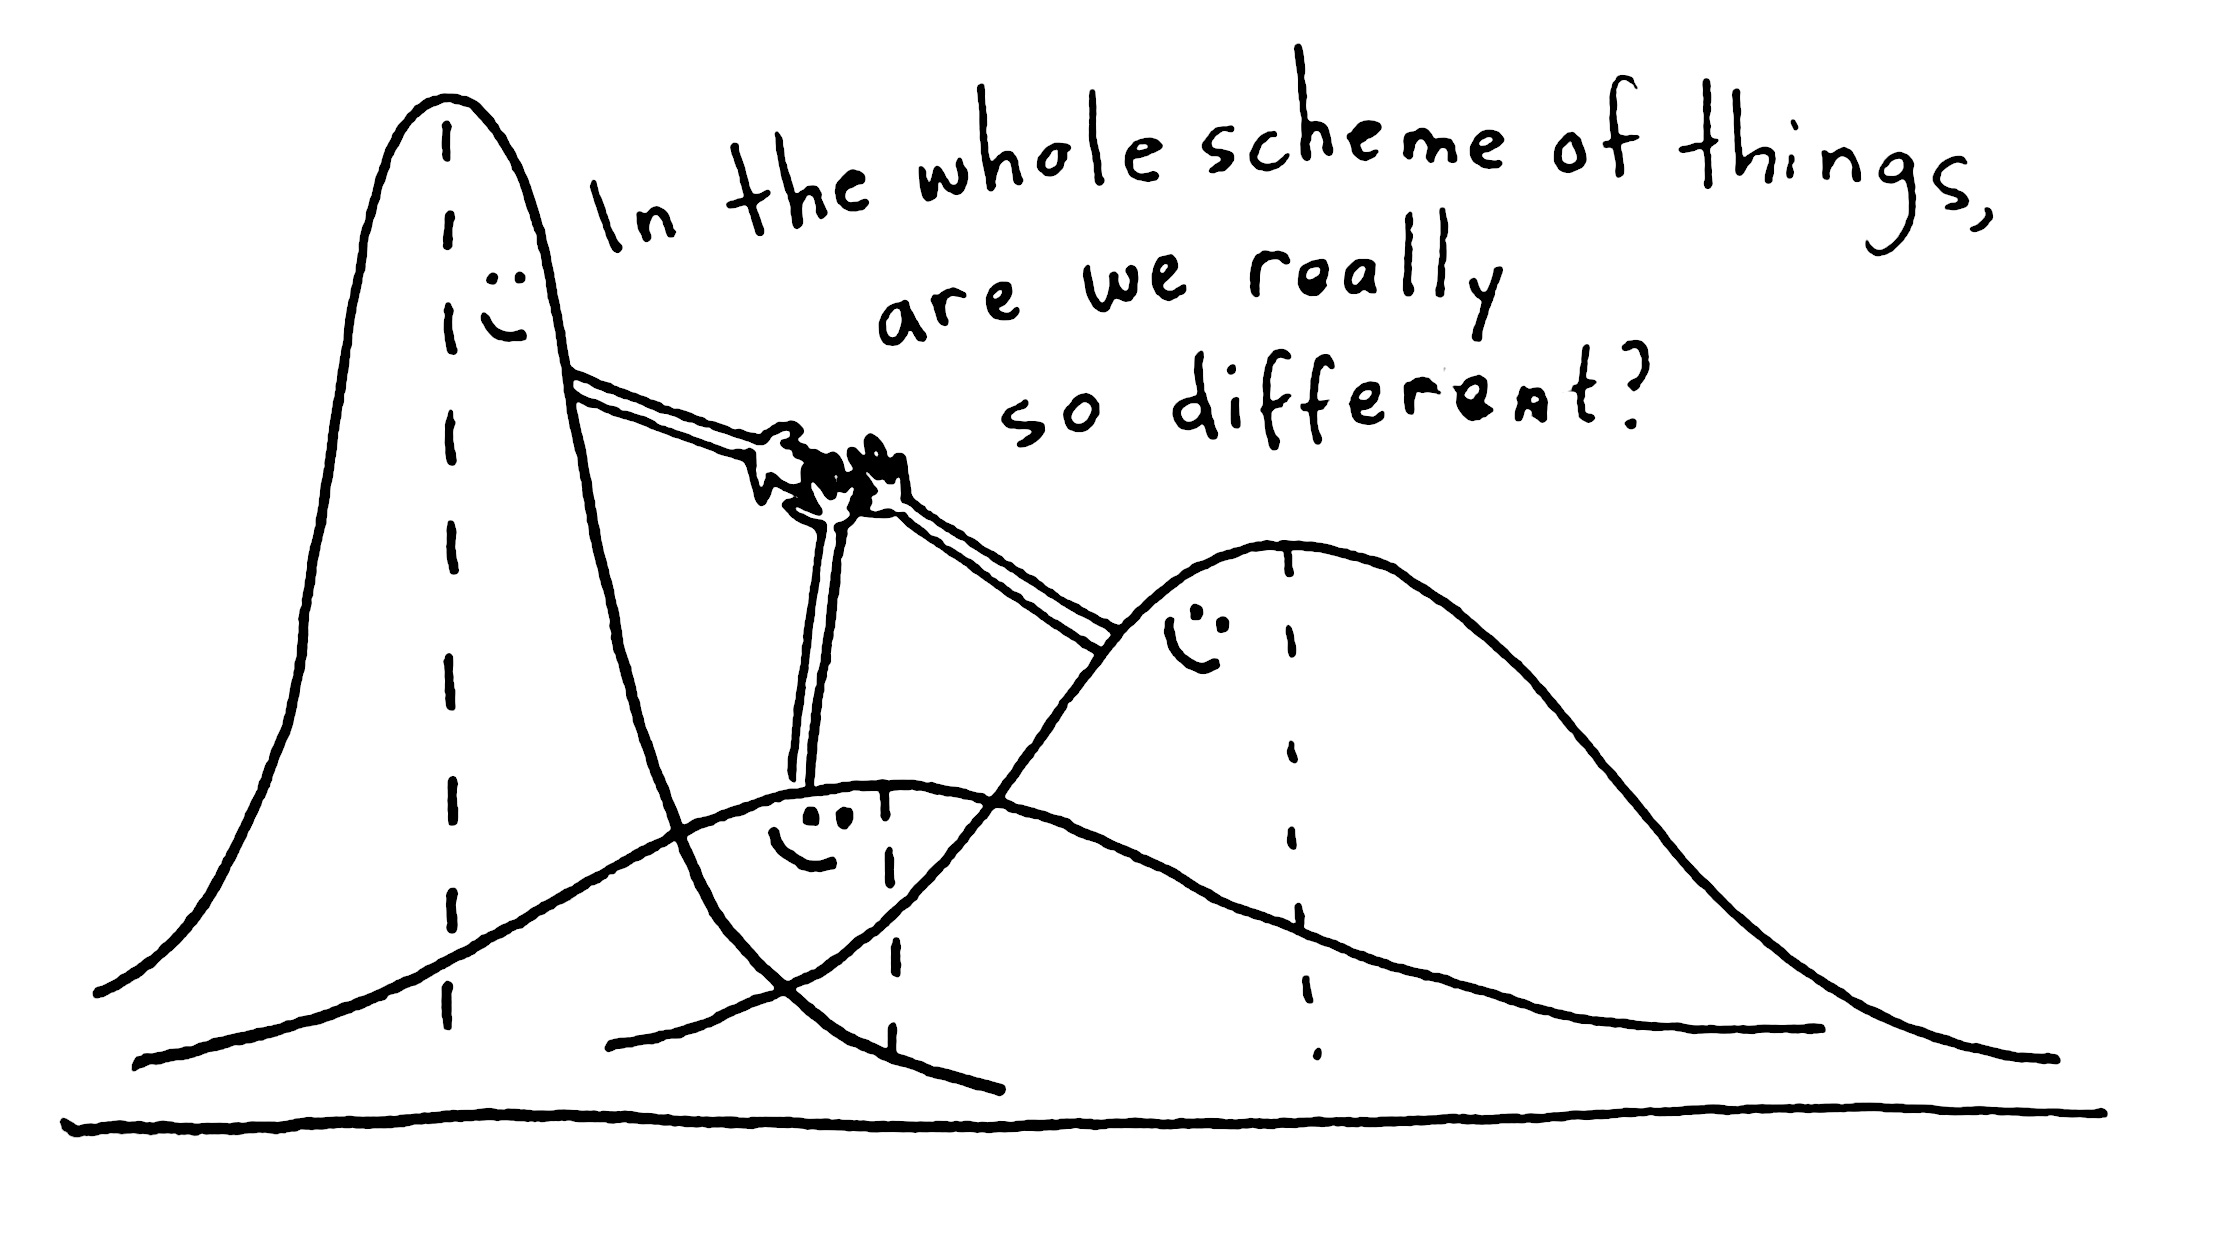
\includegraphics[width=\linewidth]{anova.jpg}
\end{frame}
\section{выбор теста}
\begin{frame}{Выбор теста}
\footnotesize
\begin{tabular}{|l|l|r|l|}
\mcrot{1}{c}{10}{тип данных и распределение} & \mcrot{1}{c}{10}{тип группы} & \mcrot{1}{c}{10}{количество групп} & \mcrot{1}{c}{0}{тест} \\ 
\hline
\parbox[t]{2mm}{\multirow{3}{*}{\rotatebox[origin=c]{90}{норм.}}} & \multicolumn{ 1}{l|}{с заданным значением} & 1 & одновыборочный t-test \\ \cline{ 2- 4}
\multicolumn{ 1}{|l|}{} & независимые & 2 & t-test для независимых выборок \\ \cline{ 2- 4}
\multicolumn{ 1}{|l|}{} & зависимые & 2 & парный t-test \\ \cline{ 3- 4}
\hline
\parbox[t]{2mm}{\multirow{3}{*}{\rotatebox[origin=c]{90}{не норм.}}} & \multicolumn{ 1}{l|}{с заданным значением} & 1 & критерий Уилкоксона \\ \cline{ 2- 4}
\multicolumn{ 1}{|l|}{} & независимые & 2 & критерий Манна-Уитни \\ \cline{ 2- 4}
\multicolumn{ 1}{|l|}{} & зависимые & 2 & критерий Уилкоксона \\ \hline
\parbox[t]{2mm}{\multirow{3}{*}{\rotatebox[origin=c]{90}{категор.}}} & \multicolumn{ 1}{l|}{с заданными частотами} & 1 & биномиальный тест, χ² \\ \cline{ 2- 4}
\multicolumn{ 1}{|l|}{} & независимые & 2 & χ² с поправкой Йейтса, Фишер, Крамер \\ \cline{ 2- 4}
\multicolumn{ 1}{|l|}{} & зависимые & 2 & критерий Мак-Нимара \\\hline
\end{tabular}\\
\vfill
Если количество групп превышает 2, то с используют многовыборочные тесты: ANOVA (и всякие варианты ANCOVA, MANOVA, MANCOVA), критерии Краскела-Уоллиса, критерий Фридмана, Q-критерий Кокрена и χ² с поправкой на правдоподобие.
\end{frame}
\section{послесловие}
\begin{frame}{Величина эффекта (effect size)}
В статье \citep{sullivan12} приводится ряд аргументов в пользу того, что следует приводить не только p-value, но и величину эффекта:
\begin{itemize}
\mytem величина эффекта —  основной результат квантитативного исследования, p-value лишь говорит о том, что эффект с некоторой вероятностью есть
\mytem при работе со значительными выборками статистические тесты всегда будут давать статистическую значимость, даже если величина эффекта незначительна
\end{itemize}
Существует множество показателей, оценивающих величину эффекта, например при помощи функции \scriptsize\verb"cohensD"\normalsize\ пакета \scriptsize\verb"lsr"\normalsize\ можно посчитать Cohen’s $d$ (\href{http://rpsychologist.com/d3/cohend/}{\alert{здесь доступна визуализация}}):
\begin{itemize}
\mytem маленький эффект (0.2–0.3)
\mytem средний эффект (около 0.5)
\mytem сильный эффект (>0.8)
\end{itemize}
\end{frame}
\begin{frame}{p-value очень много ругают}
\begin{itemize}
\mytem за то, что его очень часто понимают неправильно\\ \citep{gigerenzer04}, \citep{goodman08}
\mytem за то, что само по себе p-value < 0.05 слабый довод\\ \citep{sterne01}, \citep{nuzzo14}, \citep{wasserstein16}
\end{itemize}
\vfill
\small
\textit{Q: Why do so many colleges and grad schools teach p = 0.05?\\
A: Because that's still what the scientific community and journal editors use.\medskip\\
Q: Why do so many people still use p = 0.05?\\
A: Because that's what they were taught in college or grad school}\\\hfill
\normalsize \citep{wasserstein16}\\
\vfill
В связи с этим, сейчас можно наблюдать
\begin{itemize}
\mytem большое обсуждение p-value vs. доверительные интервалы
\mytem  все нарастающую популярность Байесовской статистики
 \end{itemize}
\vfill
"Есть жизнь"\ и вне Пирсоновской и Байесовской статистик.
\end{frame}
\section{}
\begin{frame}
{\huge Спасибо за внимание\bigskip\\
\normalsize Пишите письма\\
agricolamz@gmail.com
\vspace{-130pt}}
\end{frame}
\begin{frame}{Список литературы}
\footnotesize
\bibliographystyle{chicago}
\bibliography{bibliography}
\end{frame}
\end{document}